\documentclass[10pt,reprint]{socc14}
\usepackage{mathptmx}
\usepackage[colorlinks,linkcolor=red,anchorcolor=blue,citecolor=green,urlcolor=black]{hyperref}
\usepackage{subfigure}
\usepackage{epsfig}
\usepackage{multirow}
\usepackage{array}
\usepackage{breqn}
\usepackage{pgfplots}
\usepackage{pgfplotstable}
\usepackage{sansmath}
\usepackage{booktabs}
\usepackage{soul}
\pgfplotsset{compat=1.5}
\DeclareGraphicsExtensions{.pdf}


\newcommand{\comments}[1]{}
\newcommand{\todo}[1]{\textit{\color{red}#1}}

%pgfplots setup
\pgfplotsset{
    %You are supposed to use append style rather than just setting
    %parameters globally so they are easier to override to special cases
    %thickness options:thin,ultra thin,very thin,semithick,thick,very thick
    every axis/.append style={
        thick,
        tick style={thick},
        tick label style={font=\small\mathversion{sans}\sffamily},
        label style={font=\small\sffamily},
        font={\small\sffamily},
        mark size=1.0
    },
    every legend/.append style={font={\small\mathversion{sans}\sffamily}}
}
\pgfplotsset{
    every mark/.append style={solid}
}
\pgfplotscreateplotcyclelist{mcolor}{%
    {blue,every mark/.append style={fill=blue},mark=*},
    {red,every mark/.append style={fill=red},mark=square*},
    {brown,every mark/.append style={fill=brown},mark=triangle*,mark size=1.5},
    {black,every mark/.append style={fill=black},mark=diamond*,mark size=1.5},
    {green!60!black,every mark/.append style={fill=green!60!black},mark=pentagon*,mark size=1.4},
    {magenta!90!black,every mark/.append style={fill=magenta!90!black},mark=star,mark size=1.5},
    {densely dashed,blue,every mark/.append style={fill=blue},mark=*},
    {densely dashed,red,every mark/.append style={fill=red},mark=square*},
    {densely dashed,brown,every mark/.append style={fill=brown},mark=triangle*,mark size=1.5},
    {densely dashed,black,every mark/.append style={fill=black},mark=diamond*,mark size=1.5},
    {densely dashed,green!60!black,every mark/.append style={fill=green!60!black},mark=pentagon*,mark size=1.4},
    {densely dashed,magenta!90!black,every mark/.append style={fill=magenta!90!black},mark=star,mark size=1.5}}

\pgfplotscreateplotcyclelist{mmark*}{
    {mark=*},
    {mark=square*},
    {mark=triangle*,mark size=1.5},
    {mark=diamond*,mark size=1.5},
    {mark=pentagon*,mark size=1.4},
    {mark=star,mark size=1.5},
    {mark=asterisk,mark size=1.5},
    {mark=+,mark size=1.5},
    {mark=Mercedes star,mark size=1.5}}

\pgfplotscreateplotcyclelist{mline}{
    {solid,blue,every mark/.append style={fill=blue}},
    {densely dashed,red,every mark/.append style={fill=red}},
    {densely dotted,brown,every mark/.append style={fill=brown}},
    {loosely dotted,black,every mark/.append style={fill=black}},
    {loosely dashed,green!60!black,every mark/.append style={fill=green!60!black}},
    {densely dashdotted,magenta!90!black,every mark/.append style={fill=magenta!90!black}},
    {densely dashdotdotted,teal,every mark/.append style={fill=teal}},
    {loosely dashdotted,orange,every mark/.append style={fill=orange}},
    {loosely dashdotdotted,violet,every mark/.append style={fill=violet}}}

    \pgfplotsset{cycle list name=mcolor}

%\linespread{.98} % to squeeeze lines and put figures in same page
\begin{document}
\special{papersize=8.5in,11in}
\setlength{\pdfpageheight}{\paperheight}
\setlength{\pdfpagewidth}{\paperwidth}
\conferenceinfo{Submission to SoCC '14}{October, 2014, Seattle, WA, USA}
\copyrightyear{2014}
\copyrightdata{978-1-nnnn-nnnn-n/yy/mm}
\doi{nnnnnnn.nnnnnnn}
%\title{VM-Centric Deduplication with Fault Isolation for Virtual Machine Snapshot Backup }
%Collocated Snapshot Backup with VM-Centric Deduplication in the Cloud}

%with Fault Isolation 
\title{VM-Centric Snapshot Deduplication for Converged Cloud Architectures}
%VM-Centric  Deduplication  with Fault Isolation for Snapshot Backup in the Cloud
\comments{
\authorinfo{Wei Zhang\and Daniel Agun\and Tao Yang}
           {UC Santa Barbara}
           {\{wei,dagun,tyang\}@cs.ucsb.edu}
\authorinfo{Hong Tang}
           {Alibaba Inc.}
           {hongtang@alibaba-inc.com}
\authorinfo{Rich Wolski}
           {UC Santa Barbara}
           {rich@cs.ucsb.edu}
}
 \authorinfo{
   Wei Zhang$^{\star}$, Daniel Agun$^\star$, Tao Yang$^\star$, Rich Wolski$^{\star}$, and  
Hong Tang$^\dagger$}
   {$^\star$University of California at Santa Barbara \ \ \  
   $^\dagger$Alibaba Inc. }
%  \{wei, dagun,tyang,rich\}@cs.ucsb.edu, hongtang@alibaba-inc.com

  %{\normalsize $^\star$University of California at Santa Barbara} \ \ {\normalsize$^\dagger$Alibaba Inc.} \\

\maketitle

\begin{abstract}
Data deduplication has been widely used for cloud data backup
because of excessive redundant content. Common techniques 
perform fingerprint comparison to remove duplicates
across virtual machines.
However, fingerprint search for source-side duplicate detection is resource
intensive when the backup service for virtual machines (VMs)  is co-located with  other cloud services.
%letting a duplicate data block be shared
%by many virtual machines represents a tradeoff between
%storage efficiency and data availability.
%by many virtual machines creates data dependence and is less fault-resilient. 
%%This paper studies the impact of deduplication on 
%%fault resilidence  of virtual machine snapshots, created by data dependence  among duplicates
%%and proposes a VM-centric approach that strikes a balance between deduplication efficiency
%%and fault isolation 
This paper proposes a VM-centric backup service 
which  strikes a tradeoff for a competitive  deduplication efficiency while
using small  computing resources, suitable for running
on a converged cloud architecture that cohosts  many other services.
This VM-centric design also improves the snapshot availability  during machine failures  
and simplifies snapshot deletion.  The key techniques used are to
localize deduplication as much as possible within each 
virtual machine, guided by similarity
search, and to restrict global deduplication under popular chunks with extra replication support.
This scheme associates  underlying file blocks with one VM for most cases
and proposes an approximate method for fast and simplified snapshot deletion.
This  paper  describes an evaluation of this scheme to assess  its deduplication 
efficiency, resource usage,  and fault resilience.

% Collocating a cluster-based duplicate service with other cloud services
%   necessary to eliminate
%redundant blocks and reduce cost. Collocating a cluster-based duplicate service with other cloud services

%A cloud environment that hosts a large number of virtual machines (VMs) has
%a high storage demand for frequent backup of system image snapshots. 
%Deduplication of data blocks is necessary to eliminate
%redundant blocks and reduce cost. Collocating a cluster-based duplicate service with other cloud services
%reduces network traffic;
%however, 
\end{abstract}



\category{}{Information Systems}{Information Storage Systems}
\category{}{Distributed Architectures}{Cloud Computing}
%\category{D.2.8}{Information Systems}{Information Storage Systems}
\terms{Design, Experimentation, Performance}

\keywords
Virtual machine images, snapshot backup and deletion, source-side deduplication, cluster-based architectures

\section{Introduction}

One of emerging architectures for building cloud services
is a converged storage architecture that leverages commodity servers with software clustered storage.
The converged architecture (server plus compute in same tier) grew out of the Google model. What Google recognized is that they could leverage their software to meld multiple direct attached low-cost disks together across servers and avoid paying high margins for traditional network attached storage systems. %This(e.g. ~\cite{NutanixPaper}). 
Leading cloud platform companies such as Google, Amazon, Alibaba,
Microsoft Azure  have built a converged compute and storage infrastructure and used
a distributed file system such as Google file system~\cite{googlefs03,hdfs10}
to glue a large number of commodity servers.
% with local storage into a single cluster.
In such an environment,
%That  allows the use of scalable compute and storage, without incurring the costs and
%performance limitations associated with network storage.
each physical machine runs a number  of virtual machines 
%as  instances of a guest operating system 
and their  virtual disks are represented as virtual disk image files in the host operating system.
Frequent  snapshot backup of virtual disk images  can increase  the service reliability
and deduplication of redundant content blocks~\cite{venti02,bottleneck08}
 is necessary to substantially reduce the storage demand.
%For example, the Aliyun cloud, which is  the largest cloud service provider by Alibaba in China, 
%automatically conducts  the backup of virtual disk images to all active users every day.
%The cost of supporting a large number of concurrent backup streams is high
%because of the huge storage demand and the use of deduplication
 
%Using a separate  backup service with full deduplication support~\cite{venti02,bottleneck08}
%can effectively identify and remove content duplicates among snapshots, 
%but such a solution can be expensive. There is also a large amount of 
%network traffic to transfer  data from the host machines to the backup facility
%before duplicates are removed.

While version-based detection  has been used to  identify file  blocks that have not 
changed from the previous version of the snapshot~\cite{Clements2009,Vrable2009,TanIPDPS2011},
a popular technique for deduplicatioon is to 
conduct fingerprint  comparison and identify duplicates that exist
among all files~\cite{Guo2011,Dong2011,extreme_binning09}. 
Because of highly repetitive content in snapshots from different VMs,
many data chunks are shared by virtual machines.  
Failure of a few shared data chunks can have a 
broad effect and snapshots of these virtual machines could be affected.
The previous work in deduplication focuses on the efficiency and approximation of
fingerprint comparison, and has not addressed fault tolerance issues  together with deduplication.
Thus we seek a method that strikes a balance between fault isolation and deduplication efficiency.


The main contribution of this work is to evaluate the fault tolerance  impact of popular data blocks shared by many
virtual machines, and   propose a VM-centric approach that localizes deduplication as much as possible 
and restricts global deduplication only to a limited set of most popular blocks.
Local deduplication also uses similarity-guided elimination to improve the deduplication coverage.
Since the file system block size is normally bigger than the average data chunk size used for deduplication,
we package data chunks from the same VM into a file system block as much as possible to improve fault isolation.
Because data sharing is restricted, 
this VM-centric approach reduces the overall resource usage significantly during backup and
simplifies the snapshot deletion process. This low-resource design
is suitable when the backup service with deduplication is collocated with other services running on a shared compute and storage
cluster.  We have evaluated this VM-centric approach using  a prototype system.
% that runs a cluster of Linux machines with Xen and a standard distributed file system for the backup storage. 
%This approach localizes duplicate detection within each VM  
%By narrowing duplicate sharing within a small percent of common data chunks and exploiting their popularity,
%this scheme can afford to allocate extra replicas of these shared chunks for better
%fault resilience while sustaining competitive deduplication efficiency.


%In addition, our VM-centric design allows garbage collection to be performed in a localized
%scope and we propose an approximate deletion scheme to reduce this cost further.
%Localization also brings the benefits of greater ability to exploit parallelism so
%backup operations can run simultaneously without a central  bottleneck.
%This VM-centric solution uses a small amount of  memory while delivering reasonable deduplication efficiency. 

%Another issue considered is that
%that garbage collection after deletion of old snapshots also competes for computing resources. 
%Sharing of data chunks among by multiple VMs needs to be detected during
%garbage collection and such dependencies complicate deletion operations. 

%************** Paper sections summary
%THIS NEEDS MODIFICATION
The rest of this paper is organized as follows.
Section~\ref{sect:background} reviews the background and discusses the  design options for snapshot backup 
with a VM-centric approach. 
Section~\ref{sect:deduplication}  analyzes the tradeoff and benefits of the VM-centric approach. 
Section~\ref{sect:architecture}  describes a system implementation that evaluates the proposed techniques.
%   the benefit of our approach for fault isolation. 
Section~\ref{sect:evaluation} is our experimental evaluation that compares with other approaches.
Section~\ref{sect:conclusion}  concludes this paper.

\section{Background and Design Considerations}
\label{sect:background}

Figure~\ref{fig:collocated} illustrates a converged IaaS cloud architecture 
where
each commodity server hosts a number of virtual machines and storage of these servers
is clustered using a distributed file system~\cite{googlefs03,hdfs10}.
Each physical machine hosts multiple virtual machines.  Every virtual machine
runs its own guest operating system and accesses virtual hard disks 
stored as image files maintained by the operating system running on the
physical host. 
%The secondary storage can be cluster-based and implemented with a distributed file system~\cite{googlefs03}.   
For VM snapshot backup, file-level semantics are normally not provided.
Snapshot operations take place at the virtual device driver level, which
means no fine-grained file system metadata can be used to determine the changed data. 
In a converged setting with source-side deduplication, the resources that are used to implement snapshot
backup and deduplication are the same resources that must support cloud-hosted
VMs.  Thus the backup service collocated with 
other cloud services has to minimize its resource impact.  
%This architecture does not use a separate  backup facility for a lower cost and 
%reduces the network bandwidth consumption in transferring the raw data for backup. 
%A backup service may co-locate with other cloud services on these commodity servers and 
%stores deduplicated data  in  the storage in this cluster or in
%a separate storage cluster.


%runs a backup service and 


%As discussed earlier, co-locating a backup service on the existing
%cloud cluster avoids the extra cost to acquire a dedicated backup facility

\begin{figure}[htb]
    \centering
    %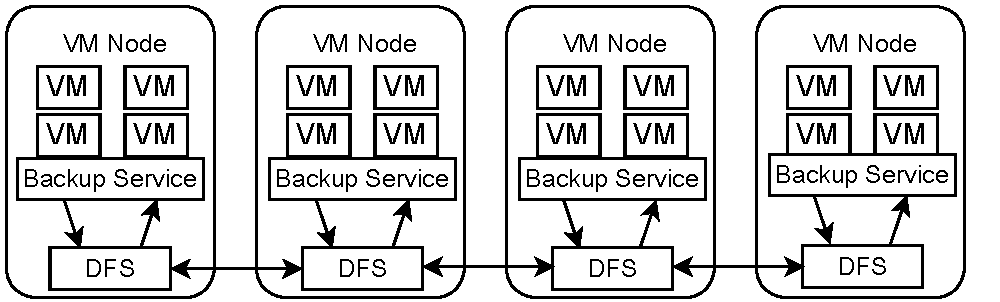
\includegraphics[width=3in]{images/colocated-arch}
    %\includegraphics[width=3in]{images/converged_arch}
    \resizebox{0.85\linewidth}{!}{
        %converged architecture diagram with a disrtibuted dedupe service, and secondary storage
\begin{tikzpicture}[thick,rounded corners,scale=0.8]\sf
	\definecolor{dfs}{gray}{0.90}
    %CDFS is the corner of the drawing (cluster with distributed file system)
    \coordinate (CDFS) at (0,0);
    %first we loop to draw 4 machines (and 4 VMs inside each machine)
    \foreach \x / \i in {0 / -1.5, 2.5 / -0.5, 5 / 0.5,8.0 / 1.5} {
        %CMAC is the coord of the current cluster machine
        \coordinate (CMAC) at ([xshift=\x cm]CDFS);
        %first draw the box around the machine
        \draw[-stealth] (CMAC) rectangle +(2.3,3) 
        %then the dots in the middle to represent more vms
        node[pos=0.5,anchor=south]{\scriptsize\ldots}
        %next the label centered near the top
        +(1.15,2.7) node[anchor=center]{\scriptsize{}Cluster Machine};
        %++(1.15,0) -- (4.9,-0.7);
        \draw[-stealth] ($(CMAC)+(1.15,0)$) -- ($(4.9,-0.7)+0.5*(\i,0)$);
        %now loop through the 4 vms we will draw
        \foreach \vmx in {0.1, 1.3} \foreach \vmy in {1,1.7} {
            \coordinate (CVM) at ([xshift=\vmx cm,yshift=\vmy cm]CMAC);
            %first draw the vm rectangle
            \draw[rounded corners=0.1cm] (CVM) rectangle +(0.8,0.6)
            %then draw a label node in the middle of it
            %the nodes is 50% along the line between the last two points
            %  (i.e. the diagonal of the rectangle)
            node[pos=0.5]{VM};
        }
    }
	\node at ([xshift=7.67cm,yshift=1.75cm,align=center,anchor=center]CDFS) {$\cdots$} ;
    %now we draw the distrubuted files systems across the VMs
    \draw[fill=dfs] ([xshift=0.1cm,yshift=0.1cm]CDFS) rectangle +(10.1,0.8) node[midway]
    {Source-side deduplication};
    \draw[fill=dfs] ([xshift=2.1cm,yshift=-1.5cm]CDFS) rectangle +(6.1,0.8) node[midway]
    {Secondary Storage};
\end{tikzpicture}

        %\includegraphics{figures/converged_arch}
    }
    \caption{VM snapshot backup running on a converged cloud cluster.}
    \label{fig:collocated}
\end{figure}

File backup systems have been developed to use fingerprints generated for
data ``chunks''  to identify duplicate
content~\cite{venti02,Rhea2008}.  In a simple implementation,
it is expensive to compare a large number of 
fingerprints
so a number of techniques have been proposed to improve duplicate identification. 
For example, the data domain method ~\cite{bottleneck08} 
uses an in-memory Bloom filter to identify non-duplicates and a prefetching cache for potential
duplicates that might hit in the future.
%An improvement to this work with parallelization is in ~\cite{MAD210,DEBAR}.
%Approximation techniques are studied in~\cite{extreme_binning09,Guo2011,WeiZhangIEEE}  
%to reduce memory requirements at the cost of some loss of deduplication
%efficiency.
Additional inline deduplication and  approximation techniques
are studied in ~\cite{extreme_binning09,sparseindex09,Srinivasan2012,WeiZhangIEEE}.  
%and a parallel batch solution for cluster-based deduplication is 
%studied in ~\cite{WeiZhangIEEE}. 
% \comments{
% All of the above approaches have focused on optimization of deduplication
% efficiency or speed, and none of them have considered the impact
% of deduplication on fault resilience in a cloud environment.  To do so, we
% examine the following properties of VM snapshot deduplication for converged
% IaaS architectures.
% }
%considered in this paper.
%Our consideration is discussed below.
%VM dependence minimization during deduplication and file system block management.

Even with these optimization and approximation techniques, resource usage such as memory  for deduplication
is still extensive for a shared cloud cluster.  
For example, in the experiments discussed in Section~\ref{sect:evaldedup}, 
the raw snapshot data has a size of 1,000TB on 100 physical machines that host VMs,
cross-machine fingerprint comparison using Bloom filter and approximated routing~\cite{bottleneck08,Dong2011} 
still needs several gigabytes of memory per machine. This can impact other primary cloud services sharing the same
computing resource. Our objective is to have an approximation scheme 
which uses no more than a few hundred megabytes of memory during normal operation.
Thus the  desired ratio of raw data to memory ratio is from 100K:1 to 30K:1.
Our proposed scheme achieves 85K:1
and this ratio is about the same as the number of machines increases.

Index sampling with a prefetch cache  is proposed 
in~\cite{Guo2011} for efficient single-machine deduplication. 
This scheme uses 25GB memory per 500TB of raw data
and thus the raw data to memory ratio is 20K:1. The scheme proposed in this paper 
uses three times less memory. We have not incorporated this index 
sampling technique because it is difficult to extend 
for a distributed architecture.  To use a distributed memory version 
of the sampled index, every deduplication
request may access a remote machine for index lookup and the overall overhead 
of access latency for all requests is significant.

% \comments{
% For example, the
% sampled index with prefetching, proposed  by Guo and Efstathopoulos\cite{Guo2011},
% uses 5GB memory space for 100TB of raw data even the compressed data size
% is about 5TB. It is fairly typical for
% a physical machine with terabytes of disk storage and tens of gigabytes of memory
% to support  more than 20 VMs and 10 snapshots per VM and can require  over 100TB of raw space
% even the actual storage space need is about 5TB assuming 20:1 compression ratio with deduplication.
% It is not easy  to adopt the sampled index method  for a distributed architecture
% and every deduplication request may access a remote machine for index lookup and the overall overhead of access latency
% for all requests can be significant.
%  In general
% with a cluster of machines in a cloud cluster, there will be more memory requirement per machine such as a
% fingerprint cache, for cross-machine fingerprint comparison~\cite{bottleneck08,Dong2011} and a deduplication
% task often needs several gigabytpes of memory, which impacts other cloud services sharing the computing resource.
% }

While deduplication reduces storage cost, it creates an artificial data dependence among VMs: when a shared data chunk
is lost in the storage, all VMs that refer such chunks after deduplication face a data loss.
The work in ~\cite{Reliability06} identifies such an issue in file systems 
and uses more replication for data shared by more files,
and we will adopt this idea.
When the backup storage is implemented using a distributed file system such as Hadoop and 
Google file system~\cite{googlefs03},  
the file system block  size is often chosen to be large (e.g. 64MB). On the other hand, 
deduplication implementations~\cite{Guo2011,extreme_binning09,bottleneck08,Jin2009,Dong2011}
 typically use smaller chunk sizes (e.g. 4K bytes).
Thus we need to address  the size gap between file system blocks and chunks.  
%in adding more replications for popular chunks. 

%Another disadvantage of cross-VM sharing is that it complicates
Snapshot deletion 
%which is the garbage collection in VM environment
occurs frequently because snapshots expire regularly
and reference counting is required to identify chunks that are no loner used.
%Several well developed garbage collection methods do not apply to the
%converged virtualized architecture due to various environment and resource limitations:
Grouped mark-and-sweep~\cite{Guo2011} is effective for deletion by tracking
the dependencies from data containers to metadata groups, but still it carries
a significant cost in a cloud cluster. This is because any data chunk can still be
used by a large number of VMs, and there are multiple rounds of extensive I/O involved
to scan through the meta data of snapshots to check if a chunk is referenced or not.
As the number of machines increases, the I/O cost becomes more expensive.
% and  we show  such that only a subset of
%metadata needs to be scanned in order to reclaim the garbage in any given data container.
%However, data in VM environment tend to be highly dedupable which means
%such dependency could be extensive, therefore scanning a large subset of metadata still carries a significant cost,
% especially in a distributed setting.
Perfect hashing~\cite{Fabiano2013} provides a memory efficient way to represent a large set of
hashes in a compact form, however, it still requires the scanning of all data hashes before any 
garbage collection could begin, which limits its application to an offline batch process. 
In addition, it requires a centralized location
to store the hashing result which is still too big to be held in a converged architecture.


\comments{
Our previous work on parallel deduplication~\cite{zhangusenix13} is a low-cost
solution, but it is not an inline solution and th backup for all VMs needs to be conducted
around the same time. 
It does not address  snapshot deletion and file system block packaging for fault tolerance. 
}

Our previous work on parallel deduplication~\cite{zhangusenix13,WeiZhangIEEE} 
is not a comprehensive VM-centric solution and does not address  snapshot deletion and file system block 
packaging for fault tolerance.  The work in ~\cite{zhangusenix13} is a low-cost
solution, but requires all backups for each day to occur at the same time and is less flexible than the approach presented here.



% a low cost solution, but it not an inline solution and 
%the backup for all VMs needs to be conducted
%around the same time. 

%Cross-VM chunk sharing also complicates 
% Snapshot deletion occurs frequently since  snapshots expire regularly
% and reference counting is required to identify chunks that are no longer used.
% The grouped mark-and-sweep approach~\cite{Guo2011}
% is effective for deletion, but still carries a significant cost, especially in a distributed
% setting.   This is because any data chunk can be used by any snapshot
% of virtual machines in a large cloud cluster and there are multiple rounds of  extensive I/O involved
% to scan through the metadata of snapshots to determine if a chunk has been used or not.
% As the number of virtual  machines increases, the cost becomes even worse.
%~\cite{Guo2011,Fabiano2013}  
%to count if a data chunk is still shared by other snapshots. 


%still significant
%especailly for a distributed setting.


% \comments{
% \paragraph*{Local versus Global Deduplication} --
% If deduplication is implemented strictly in the storage system,
% a data chunk is compared with fingerprints collected from all VMs during
% the deduplication process, and only a small number of
% copies of duplicates are stored in the storage.  This sharing
% artificially creates hidden data dependencies among different VMs owned by
% different
% who
% contract for isolation
% by the IaaS cloud platform.  That is, the unit of failure visible to the cloud
% user is the VM, but the unit of sharing in a deduplicated data store is the
% data chunk.

% Indeed, the greater the deduplication efficiency, the less
% the data redundancy is maintained, and the greater the ``hidden'' data
% dependence between VMs that must be hosted as if they were physically isolated.
% Thus,
% restricting deduplication to be local to each VM (but across snapshots)
% aligns the units of storage with the isolation properties guaranteed by the
% cloud at the possible expense of storage efficiency.
% %Localizing the impact of deduplication can increase fault isolation and resilience.
% %Thus from the fault tolerance point of view,  duplicate sharing among multiple VMs is
% %discouraged.


% Additionally, storage efficient deduplication can be computationally expensive
% to implement in a distributed setting.  In particular, duplicate detection is
% logically a ``global'' operation over all data chunks
% under consideration.
% By localizing duplicate search, the computational requirements
% for deduplication can be reduced, because fewer chunks must be compared.
% Further, deduplication of VMs can easily be implemented in
% parallel.

% Another disadvantage of cross-VM sharing is that it complicates
% snapshot deletion, which occurs frequently because snapshots expire regularly.
% Several well developed garbage collection methods do not apply to the
% converged virtualized architecture due to various environment and resource limitations:
% Grouped mark-and-sweep~\cite{Guo2011} is an effective approach by tracking
% the dependencies from data containers to metadata groups, such that only a subset of
% metadata needs to be scanned in order to reclaim the garbage in any given data container.
% However, data in VM environment tend to be highly redundant which means
% such dependency could be extensive, therefore scanning a large subset of metadata still carries a significant cost,
%  especially in a distributed setting.
% Perfect hashing~\cite{Fabiano2013} provides a very memory efficient way to represent a large set of
% hashes in a compact form, however, it still requires the scan of all data hashes before any garbage could begin,
% which limits its application to only offline batch garbage collection. In addition, it requires a centralized location
% to store the hashing result which is still too big to be hold anywhere in a converged architecture.


% Another disadvantage of cross-VM sharing is that it complicates
% snapshot deletion, which occurs frequently because snapshots expire regularly.
% Several well developed garbage collection methods do not apply to the
% converged virtualized architecture due to various environment and resource limitations:
% Grouped mark-and-sweep~\cite{Guo2011} is an effective approach by tracking
% the dependencies from data containers to metadata groups, such that only a subset of
% metadata needs to be scanned in order to reclaim the garbage in any given data container.
% However, data in VM environment tend to be highly dedupable which means
% such dependency could be extensive, therefore scanning a large subset of metadata still carries a significant cost,
%  especially in a distributed setting.
% Perfect hashing~\cite{Fabiano2013} provides a very memory efficient way to represent a large set of
% hashes in a compact form, however, it still requires the scan of all data hashes before any garbage could begin,
% which limits its application to only offline batch garbage collection. In addition, it requires a centralized location
% to store the hashing result which is still too big to be hold anywhere in a converged architecture.

% %to count if a data chunk is still shared by other snapshots.

% Thus,
% localizing deduplication to the VM can align fault isolation properties and
% guarantees, improve the computational efficiency of snapshot maintenance, and
% simplify snapshot deletion over non-localized approaches at the possible
% expense of storage efficiency.

% %minimize data sharing and simplify deletion while sacrificing
% %deduplication efficiency, and  can facilitate parallel execution of snapshot operations.
% \paragraph*{Units of Storage versus Units of Sharing} --
% The file system block  size in a distributed file system such as
% the Hadoop file system and the Google file system~\cite{googlefs03}
% is large (e.g.  64MB) so as to optimize file system performance
% for big data.
% Typically, deduplication implementations use smaller block sizes (4K bytes to
% 8K bytes on average~\cite{Jin2009}).
% In addition to the failure correlation that cross-VM data deduplication can
% introduce, disk block sharing of data chunks is another potential source of
% hidden data dependence.
% Thus a VM-centric solution should consider how data chunks from VMs are
% distributed among large file system blocks when a large-scale distributed file
% system is used for snapshot storage.

% %a minimum association of FSBs to VMs in the packaging
% %process. By minimizing this association we can improve fault tolerance by
% %reducing the number of VMs affected when storage nodes are lost.


% \paragraph*{Moderating Resource Usage} --
% In a converged setting, the resources that are used to implement snapshot
% backup and deduplication are the same resources that must support cloud-hosted
% VMs.  Thus the backup service must share the resources available to
% other cloud services as illustrated in Figure~\ref{fig:collocated},
% and has to minimize its impact on user-deliverable performance.
% %The key resource for global comparison  is memory for storing the fingerprints.
% %During snapshot deletion, reference counting for all unique blocks used in all VMs requires a significant resource usage
% %too.  Thus we seek for the low-profile techniques with approximation and low resource consumption.

% }

% \comments{
% With the above  considerations in mind, we propose a
% VM-centric approach (called VC)
% for a co-located backup service that has a resource usage profile
% suitable for use with converged cloud architectures.
% This compares the traditional deduplication approach {\em VM-oblivious} (VO)
% which manages duplicate data chunks without consideration of VMs.
% We discuss our key ideas and design in the next section.
% %Our key idea is to simplify deduplication management and
% }
% \comments{
% In designing a VC deduplication solution, we have considered and adopted some of
% the following previously-developed techniques.
% 1) {\em Changed Block Tracking}.
% VM snapshots can be  backed up  incrementally by identifying data segments that have
% changed from the previous version of the snapshot~\cite{Clements2009,Vrable2009,TanIPDPS2011}.
% Such a scheme  is  VM-centric since deduplication is localized to the snapshot
% history for each VM.
% %We are seeking for a tradeoff since
% %global signature comparison can deliver additional compression~\cite{Guo2011,Dong2011,extreme_binning09}.
% 1) {\em Stateless  Data Routing}.
% One approach to scalable duplicate comparison is to use content-based hash
% partitioning called stateless data routing by Dong et al.~\cite{Dong2011}.
% Stateless data routing divides the deduplication work with a similarity approximation. This work
% is similar to Extreme Binning by Bhagwat et al.~\cite{extreme_binning09} and
% each request is routed  to a machine which holds
% a Bloom filter  or can fetch on-disk index for additional comparison.
% While this approach is VM-oblivious, it motivates us to  use  a combined signature of a dataset to narrow
% VM-specific local search.
% 3) {\em Sampled Index for Memory Parsimony}.
% One effective approach that reduces memory usage is
% to use a sampled index with prefetching, proposed  by Guo and Efstathopoulos\cite{Guo2011}.
% The algorithm is VM oblivious and it is not easy  to adopt for a distributed architecture.
% To use a distributed memory version of the sampled index, every deduplication request
% may access a remote machine for index lookup and the overall overhead of access latency for all requests
% can be significant.

% We will first discuss and analyze the integration of the VM-centric deduplication strategies with fault isolation
% and discuss snapshot deletion support, then present an implementation design.
% }

\section{VM-centric Snapshot Deduplication}
\label{sect:deduplication}


With the considerations discussed in the previous section, we propose a
VM-centric approach (called VC)
for a co-located backup service that has a resource usage profile
suitable for use with converged cloud architectures.
This compares the traditional deduplication approach {\em VM-oblivious} (VO)
which manages duplicate data chunks without consideration of VMs.
Section~\ref{sect:vc-strategies} discusses  our key ideas and design for duplicate detection.
Section~\ref{sect:delete} presents  a simplified snapshot deletion with  the VM-centric approach.

\subsection{VM centric  strategies}
\label{sect:vc-strategies}

We describe our overall deduplication approach as consisting of three
complementary strategies: VM-local
duplicate search, global deduplication using popular chunks, and 
VM-centric file system block management. 
\begin{itemize}
\item 
\textbf{Cross-VM global deduplication using popular chunks} --
We separate the deduplication within a VM and cross VMs
and simplify the cross-VM deduplication while maximizing the inter-VM deduplication efficiency  as much as possible.
This is because global deduplication that detects the appearance of a chunk 
in any VM requires a substantial resource for fingerprint comparison.
To simplify cross-VM deduplication, we restrict the search scope of deduplication within the top $k$ 
most popular items. This popular data set is called the \textbf{PDS}. 
%This step accomplishes the canonical global fingerprint lookup using a popular fingerprint index.
 \begin{figure}
 \centering
  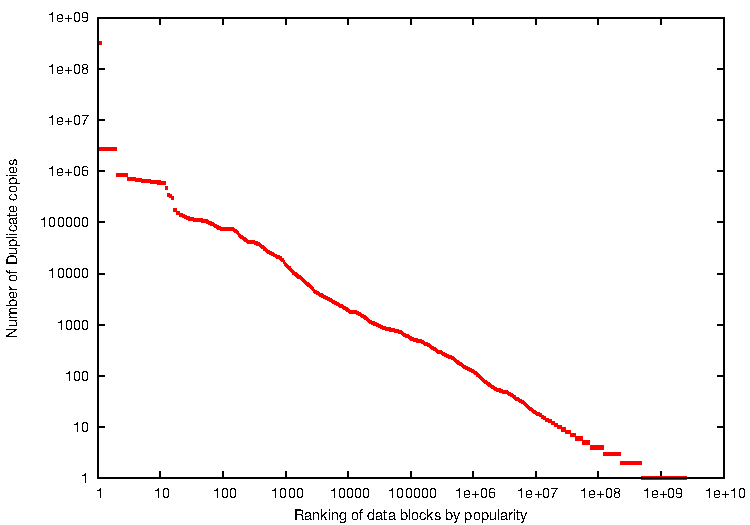
\includegraphics[width=3.25in]{figures/zipf_count_rank.pdf}
 \caption{Duplicate frequency versus  chunk ranking in a log scale after local deduplication.}
 \label{fig:Datazipf}
 \end{figure}


% {\it [Need to find a place to put these numbers in: Total number of chunks 
% in 350 snapshots: 1,546,635,485. 
% Total number of chunks after localized dedup: 283,121,924. Total number of unique chunks: 87,692,682.]}
The observation that motivates us to use the PDS
is that for those chunks that appear in different VMs, the top $k$ most popular items
dominate the appearance distribution.  
Figure~\ref{fig:Datazipf} shows the distribution of chunk popularity for a data trace 
from Alibaba with 2500 VMs discussed in Section ~\ref{sect:evaluation}.
We define chunk popularity as the number of unique copies of the chunk in the data-store,
i.e., the number of copies of the chunk after local deduplication.
%the distribution of chunk popularity~\cite{WeiZhangIEEE} 
%based on a production data trace from Alibaba with over 2500 VMs.
The distribution from this figure is Zipf-like. 
Let  $\sigma$ denote as the percentage of unique data chunks belonging to PDS and 
from the evaluation in Section~\ref{sect:evaluation}, we find that
$\sigma$ with about  2\% can deliver a fairly competitive deduplication efficiency.
%$\sigma$ with about  range of 2 to 4\% can deliver a fairly competitive deduplication efficiency.
%For example,
%with top 2\% of the most popular chunks stored in PDS, up-to 40\% of the raw backup 
%data can be eliminated by fingerprint lookup in PDS index.

%when restricting fingerprint comparison within a VM uses
%only a small amount of resource. 
%ehat the local deduplication has removed most of the duplicates.
%There are fewer deduplication opportunities across VMs while the memory and network
%consumption for global comparison is more expensive.
%Thus our approximation is that the global cross-VM fingerprint comparison only searches for the top $k$
%most popular items. 
PDS  can be computed in an offline manner periodically, e.g., on a monthly basis.
%Once the popularity of all data chunks is collected, the system only maintains the top $k$
%most popular chunk fingerprints (called \textbf{PDS index}) in a distributed shared memory.  
%These top chunks are shared among multiple VMs and  since $\sigma$ is relatively small, 
%we can afford to provide extra replicas for these popular chunk data to enhance the fault resilience.
%Compared to a preliminary solution which  uses data popularity~\cite{WeiZhangIEEE}, 
%this paper provides  a more comprehensive scheme with  improved deduplication efficiency and fault tolerance, and
%analytic design guidance. 
% Figure~\ref{fig:Datazipf} illustrates the distribution of chunk popularity based on a data trace from Alibaba with over 2500 VMs.
% The distribution is zipf like and popular chunks are dominating the large portion of data chunks.
% We denote $\sigma$ as the percentage of unique data chunks belonging to PDS and from the evaluation we find that
% $\sigma$ with a range of 1 to 4\% can deliver a fairly competitive deduplication efficiency.
Compared to ~\cite{bottleneck08}, the fingerprint index  size is reduced by $100-\sigma$ percentage
(e.g. 98\% with $\sigma=2\%$)
and the searchable fingerprint space  becomes very small under the popularity constraint.  
The fingerprint-guided distributed mapping in ~\cite{extreme_binning09,Dong2011} narrows
the search scope of each data chunk, but it does not reduce th total amount of searchable fingerprints
used for the entire deduplication. 
%In comparison we only focus on top popular chunks among VMs and this
%significantly reduces the total amount of  searchable fingerprints. 

\comments{
We have not adopted the index sampling in \cite{Guo2011} because its extension for
for a distributed architecture is difficult.  To use a distributed memory version of the sampled index, every deduplication 
request may access a remote machine for index lookup and the overall overhead of access latency for all requests
can be significant.
}
\item 
\textbf{VM-specific duplicate search optimization} --
While cross-VM deduplication is simplified, we intend to optimize the VM-specific deduplication 
under a reasonable memory consumption
 to make up the loss of deduplication opportunities due to the cross-VM popularity constraint.
%Fingerprint lookup within a VM does not require a signficant  amount of memory resource.
We start with the standard version-based detection~\cite{Clements2009,Vrable2009}
to identify changed content with dirty bits in a coarse grain segment level.
%In our implementation 
%the segment size is 2MB
%and the device driver is extended to support tracking changed segments using a dirty bitmap. 
The reason to choose a coarse grain segment level is that 
since every write for a segment will touch a dirty bit, the device driver maintains dirty bits in 
memory and cannot afford a small segment size.
It should be noted that dirty bit tracking is supported or can be easily implemented in 
major virtualization solution vendors. 
%% this method is so widely-used and easy to understand, everyone include Pure Storage has it, I feel no need to explain further.
%{
%For example,
%the VMWare hypervisor has an API to let external backup applications know 
%the changed areas since last backup. 
%The Microsoft SDK provides an API that allows external applications to monitor 
%the VM's I/O traffic and implement such changed block tracking feature.
%}

\begin{figure}[htbp]
  \centering
  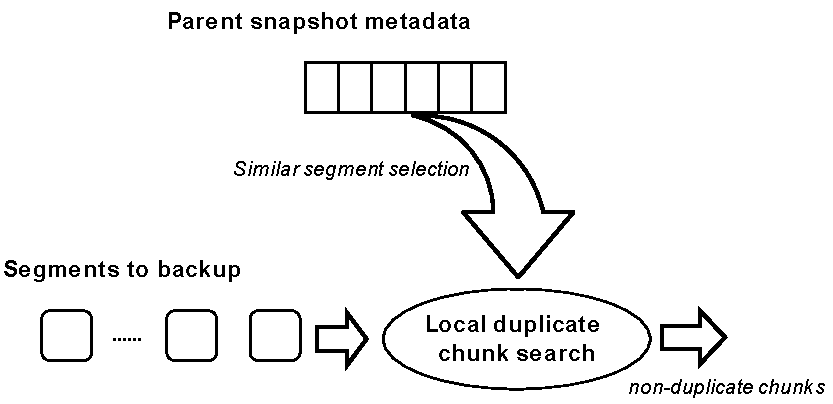
\epsfig{file=images/mh_local_dedup.pdf, width=3.25in}
  \caption{Similarity-guided local duplicate detection}
  \label{fig:local_dedup}
\end{figure}

Since the previous work typically uses a non-uniform chunk size 
with an average of 4KB or 8KB for the best deduplication 
effectiveness~\cite{Guo2011,extreme_binning09,bottleneck08,Dong2011},
we conduct additional local similarity guided deduplication 
by comparing chunk fingerprints of a dirty segment on a snapshot 
with those in  {\em potentially similar} segments from its parent snapshot. 
We consider a parent  segment is  potentially similar to the current dirty segment if 1) the parent segment
is at the same offset as the current segment.
2) the signature of these segments is the same.
The signature of a segment is defined as the minimum value of all its chunk fingerprints 
computed during backup and is recorded in the snapshot metadata (called recipe). 
%Note that this definition of content similarity is an approximation~\cite{resemblance97}.  
This signature definition is motivated by the previous work for similarity-based routing in parallel
deduplication~\cite{extreme_binning09,Dong2011} and near duplicate detection~\cite{shingling97}. 



When processing a dirty segment,
its  similar segments can be found easily from the
parent snapshot metadata.  Then metadata of the similar segments is loaded to memory,
which contain chunk fingerprints to be compared.
To control the time cost of search, we set a limit on the number of  similar segment recipes to be fetched. 
% Then,
%given a set of data chunks within a dirty segment,  we compare  these chunk fingerprints
%with those in similar segments.  
For example, assume that  a segment is of size  2MB, 
its segment recipe is roughly 19KB which contains about 500 chunk fingerprints and other chunk metadata.
By limiting at most 10 similar segments to search, the amount of memory for maintaining those 
similar segment recipes is 190K, which is insignificant. 
%compared to other memory requirements.

%As part of our local duplicate search we also compare the current segment
%against the parent segment at the same offset.

\item 
\textbf{VM-centric file system block management} --
When a chunk is not detected as a duplicate to any existing chunk, this chunk will be written
into a file system block.  
In addition to the fact that a distributed file system block is often
configured to be much  larger than a chunk, a number of chunks can be combined together
and compressed further using a standard compression method such as LZO. 
Thus a  backend file system block contains a large number of compressed chunks.
%We manage this accumulation process using a log-structured storage scheme built
%on a distributed file system discussed in Section~\ref{sect:architecture}.
%Non-PDS chunks from the same VM are stored in one append store. 
We set the following two constraints in composing chunks for a file system block:
1) Each file system block is either dedicated to non-PDS chunks, or to PDS-chunks.
2) A non-PDS file system block is only associated with one VM.

Restricting the association with one VM improves fault isolation when some file blocks are lost during 
storage failures. 
In addition, storing PDS chunks separately from non-PDS chunks
allows special replication handling for those popular shared data. 
%%% talk something about snapshot store advantage here? %%%
%One could try to rely on filesystem features to 
If we do not separate the
popular chunks from the less-popular, the popular chunks are dispersed across
all of the filesystem blocks in the storage system and we would have
to add extra replications for {\em all} file blocks in order to   follow the popularity-driven replication idea 
from ~\cite{Reliability06}. That reduces the storage efficiency.
%Then we cannot leverage the file system features to 
%provide extra replication to popular and shared chunks because  
%we have to add extra replication to each file block as long as it contains a popular chunk.

%factor on popular chunks. This explains why we must separate the PDS and
%non-PDS data in our system to achieve the desired $r_c/r$ ratio (though both
%can be stored on the same DFS).

%The system allows all machines conduct backups in parallel, and each machine
%conducts the backup of one VM at a time, and thus only requires a write buffer for one VM.
\end{itemize}




\subsection{Snapshot Deletion with Leak Repair}
\label{sect:delete}


\begin{figure}[htbp]
  \centering
  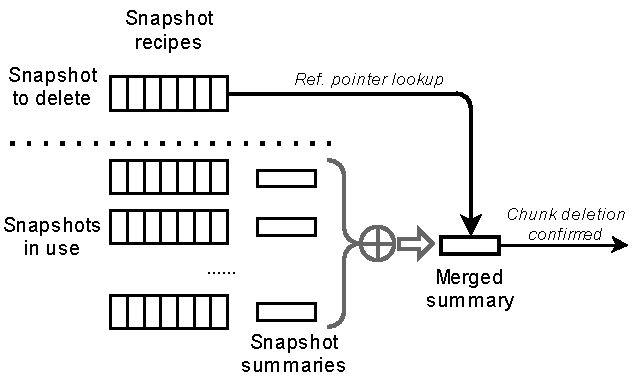
\epsfig{file=images/deletion.pdf, width=3in}
  \caption{Approximate deletion}
  \label{fig:deletion_flow}
\end{figure}

Snapshot deletions can occur frequently since old snapshots become less useful.
General deduplication complicates the deletion process because sharing of duplicates
requires a global refence counting~\cite{Guo2011,Fabiano2013} 
 to identify if  a chunk can be  safely removed without any reference.
%The complexity of our distributed environment obviates reference counting as an option,
%and While we can use the mark-and-sweep, 
%While the mark-and-sweep techniques can be used and optimization can be considered~\cite{Fabiano2013},
%it still takes significant resources to conduct reference counting every time there is a snapshot deletion.
%
%In the case of Alibaba, snapshot backup is conducted automatically and there are 
%about 10 snapshot stored for every VM customer.
% Snapshot deletion can occur frequently, for example when there is
% a new snapshot created every day,  there will usually be a snapshot expired every day to maintain
% balanced storage use. 
%In addition, cloud users expect the reduced storage usage to be reflected
%instantly, which makes it difficult to adopt some resource efficient techniques such like perfect hashing\cite{Fabiano2013}.
Since our VM-centric design restricts sharing of data chunks only to a small dataset,
we can greatly simplify the deletion process by 
focusing on  unreferenced non-PDS chunks within each VM. 
This process can be conducted by independent among VMs, and thus results in  a simpler flow control and 
lower resource usage. 
%The PDS data chunks are commonly shared among all VMs and we do not consider them
%during snapshot deletion.  The selection of PDS data chunks is updated periodically independent of snapshot deletion process.

We further propose an {\em approximate} deletion strategy to trade deletion accuracy for
speed and resource usage. Our method sacrifices a small percent of storage leakage
to efficiently identify unused chunks.
The algorithm contains three aspects.
\begin{itemize}
\item {\bf Computation for snapshot reference summary.}
Every time there is a new snapshot created,
we compute a Bloom-filter with $z$ bits as the reference summary vector for all non-PDS chunks used 
in this snapshot.
The items we put into the summary vector are all the references appearing in the metadata of the snapshot.
For each VM we preset the vector size according to  estimation of VM image size,
given $h$ snapshots stored for a VM, there are $h$ summary vectors maintained.
We adjust the summary vector size and recompute the vectors if the VM size changes substantially over time.
This can be done during the periodic leakage repair stage described below.

\item {\bf Approximate deletion with fast summary comparison.}
When there is a snapshot deletion,  
we need to identify if chunks to be deleted from that snapshot
are still referenced by other snapshots. 
This is done approximately and quickly by comparing the 
reference of deleted chunks  with
the merged reference summary vectors of other live snapshots.
The merging of live snapshot Bloom-filter vectors uses the bitwise OR operator 
and the merged vector still takes $z$ bits.
Since the number of live snapshots $h$ is limited for
each VM, 
the time and memory cost of this comparison is small, linear to the number of chunks to be deleted.

If a chunk's reference is not found in the merged summary vector, we are sure that
this chunk is not used by any live snapshots, thus it can be deleted safely.
However, among all the chunks to be deleted, 
there are a small percentage of unused chunks  which
are misjudged as  being in use, resulting in storage leakage.

\item {\bf Periodic repair of leakage}.
%[exlpain why second Bloom filter, why scan append store]
Leakage repair is conducted periodically to fix the above approximation error.
This procedure compares the live chunks for each VM with what are truly used in the VM snapshot recipes.
A mark-and-sweep process  requires a scan of the entire snapshot store.
%Our VM-centric mark-and-sweep procedure is similar to Guo\cite{Guo2011} 
%in a way that the data dependency is clearly known.
%This generally requires a scan of almost the entire snapshot store which is much more expensive than approximate deletion,
%although certain optimized algorithms may apply\cite{Przemyslaw2013}. But 
Since it is a VM-specific procedure, 
the space and time cost is relatively small compared to the tranditional mark-and-sweep
which scans snapshot chunks from all VMs.
For example, consider each reference consumes 8 bytes plus  1 mark bit. A VM that has 40GB backup data with about
10 million chunks will need less than 85MB of memory to complete a VM-specific mark-and-sweep process
in less than half an hour, assuming 50MB/s disk bandwidth is allocated.
\end{itemize}

%{\bf Discussion}
We now estimate the size of storage leakage and how often leak repair needs to be conducted.
Assume that  a VM keeps $h$ snapshots in the backup storage, creates and deletes one snapshot
every day. Let $u$ be the total number of chunks brought by the initial backup for a VM, $\Delta u$ be the average
number of additional chunks added from one snapshot to the next snapshot version. Then the total number of 
chunks stored in a VM's snapshot store is about:
\[
U = u + (h-1)\Delta u.
\]

Each Bloom filter vector has  $z$ bits for each snapshot and let $j$ be the number of hash functions used by the
Bloom filter.  Notice that a chunk may appear multiple times in these summary vectors; however, this should not 
increase the probability of being a 0 bit in all $h$ summary vectors.
Thus the probability that a particular bit is 0  in all $h$ summary vectors is  
$(1- \frac{1}{z}) ^{j U}$. 
Then the misjudgment rate of being in use  is: 
\begin{equation}
\label{eq:falserate}
\epsilon = (1-(1-\frac{1}{z})^{jU})^j.
\end{equation}

For each snapshot deletion, the number of chunks to be deleted is nearly identical to the number of
newly added chunks $\Delta u$. 
Let $R$ be the total number of runs of approximate deletion between two consecutive 
repairs. We estimate  the total leakage $L$ after $R$ runs as:
\[
L = R \epsilon \Delta u.
\]

When leakage ratio $L/U$ exceeds a pre-defined threshold $\tau$, we trigger a leak repair. Namely,

\begin{equation}
\label{eq:leakrepair}
\frac{L}{U} = \frac{R \Delta u \epsilon}{u+(h-1)\Delta u } > \tau 
\Longrightarrow R > \frac{\tau}{\epsilon}\times\frac{u + (h-1)\Delta u}{\Delta u}.
\end{equation}

For example in our tested dataset,  
$h=10$ and each snapshot adds
about 0.1-5\% of new data. Thus we take ${\Delta u}/{u} \approx 0.025$. For a 40GB snapshot, $u\approx  10$ million.
Then $U=12.25$ million.
We choose  $\epsilon = 0.01$ and $\tau=0.05$.  From Equation~\ref{eq:falserate}, 
each summary vector requires $z=10U=122.5$ million bits or 15MB. From Equation~\ref{eq:leakrepair}, 
leak repair should be triggered once for every R=245 runs of approximate deletion. 
When one machine hosts 25 VMs and there is one snapshot deletion per day per VM, there would be 
only one full leak repair for one physical machine scheduled for every 9.8 days. 
If $\tau = 0.1$ then leakage repair would occur every 19.6 days.


\section{Prototype Implementation}
\label{sect:architecture}

Our prototype system runs on a cluster of Linux machines with Xen-based VMs 
and the QFS~\cite{michael2013} distributed file system. 
%to %manage  the physical disk storage. 
All data needed for the backup service including snapshot data and metadata
%and snapshot data for backup purposes, 
resides in this distributed file system. 
One physical node hosts tens of VMs, each of which accesses its virtual machine disk image through the
virtual block device driver (called TapDisk\cite{Warfield2005} in Xen).

\subsection{Per Node Software Components} 
%\begin{figure}[htbp]
\begin{figure}[htbp]
    \centering
    %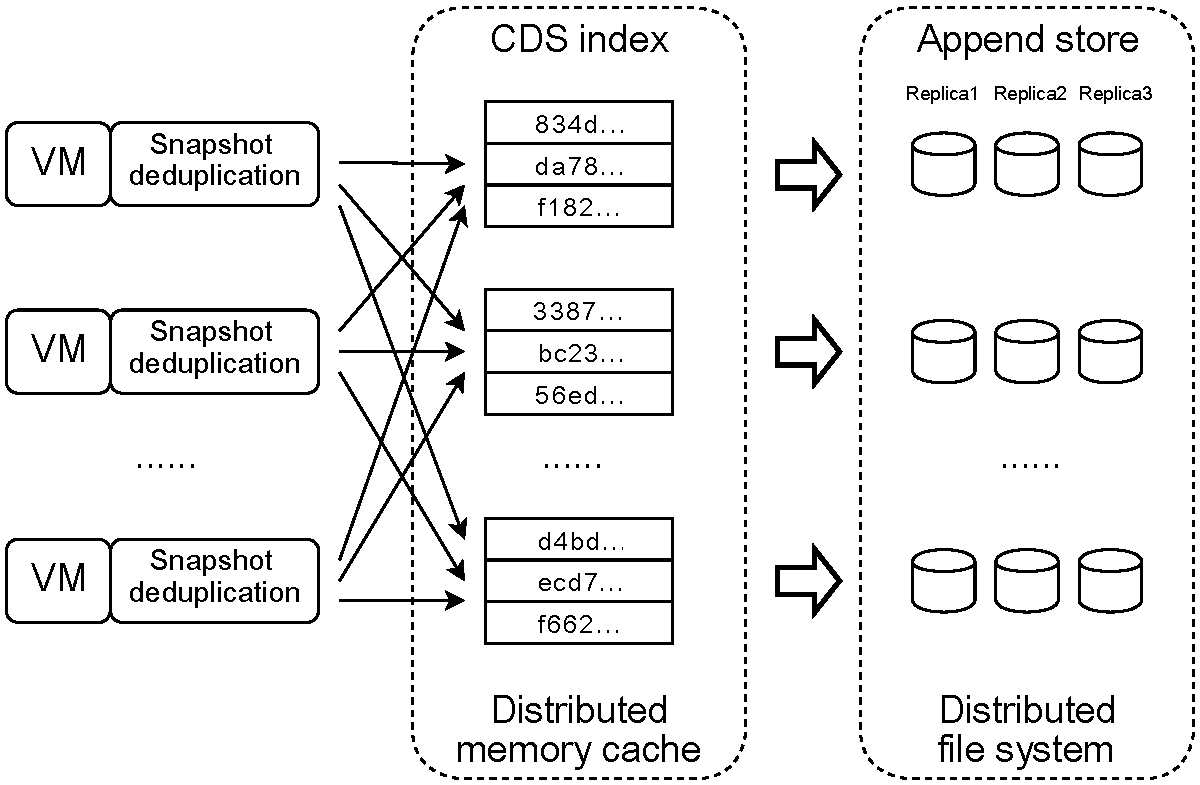
\includegraphics[width=2.75in]{images/socc_arch_cluster}
    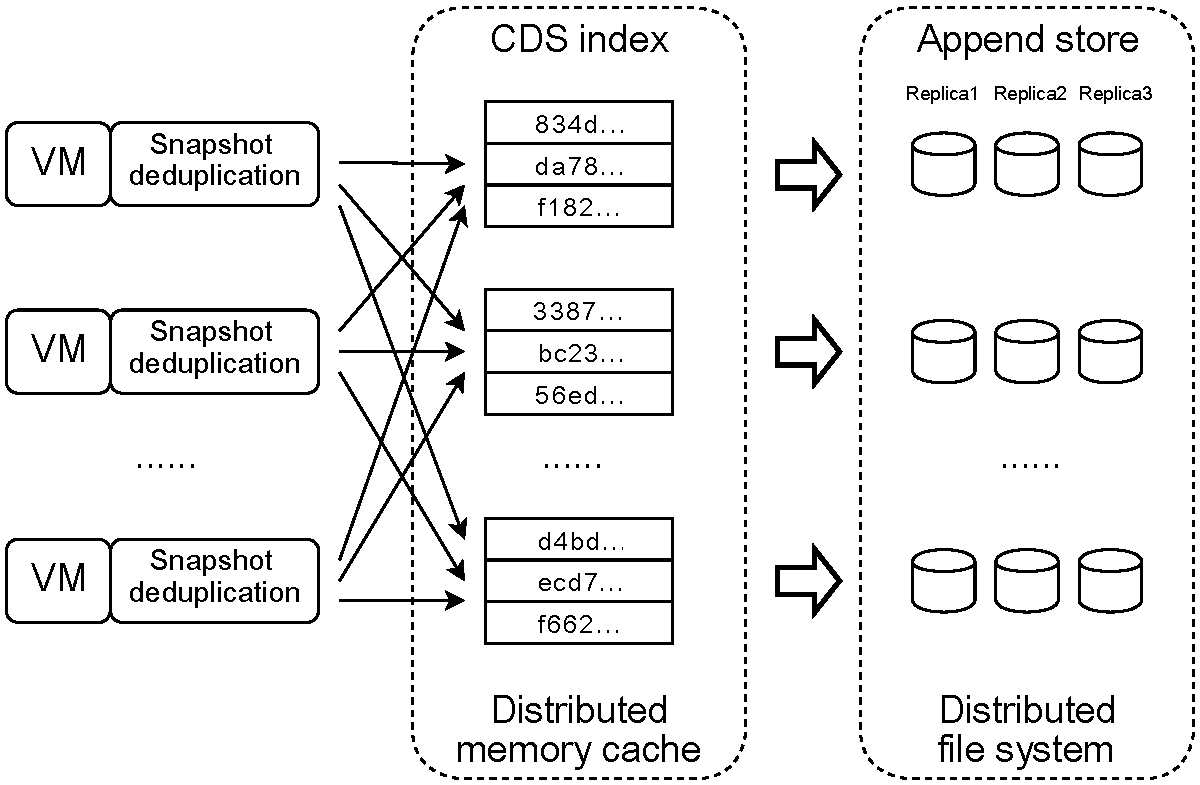
\includegraphics[width=2.2in]{images/socc_arch_cluster}
    \caption{Data flow during snapshot backup}
    \label{fig:arch_vm}
\end{figure}
As depicted in Figure~\ref{fig:arch_vm}, 
there are four key service components running on each cluster
node  for supporting backup and deduplication: 
1) a virtual block device driver, 2) a snapshot deduplication agent,
3) a snapshot store client to store  and access snapshot data,
and 4)  a PDS client to support PDS metadata access. 

We use the virtual device driver in Xen that employs a bitmap to track the changes 
that have been made to the virtual disk.
Every bit in the bitmap represents a fixed-sized (2MB) segment, indicating whether the segment
has been modified since last backup. 
Segments are further divided into variable-sized chunks (average 4KB) 
using a content-based chunking algorithm~\cite{frame05}, 
which brings the opportunity of fine-grained deduplication.
When the VM issues a disk write, the dirty bit for the corresponding segment is set
and this indicates such a segments needs to be checked during snapshot backup. 
After the snapshot backup is finished, the driver resets the dirty bit map to a clean state.
For data modification during backup, copy-on-write protection is set so that backup can continue to
copy  a specific version while new changes are recorded.
%copies a frozen version while the modification can still carry on.

The representation of each snapshot has  a two-level index data structure.
The snapshot meta data (called snapshot recipe) contains a list of segments, each of which contains segment
metadata of its chunks (called segment recipe).
In snapshot and segment recipes, 
the data structures  include references to the actual data location to eliminate the need for additional indirection.


\subsection{A VM-centric Snapshot Store for Backup Data}
\label{sect:store}
%\begin{figure}[htbp]
\begin{figure}[htbp]
  \centering
%  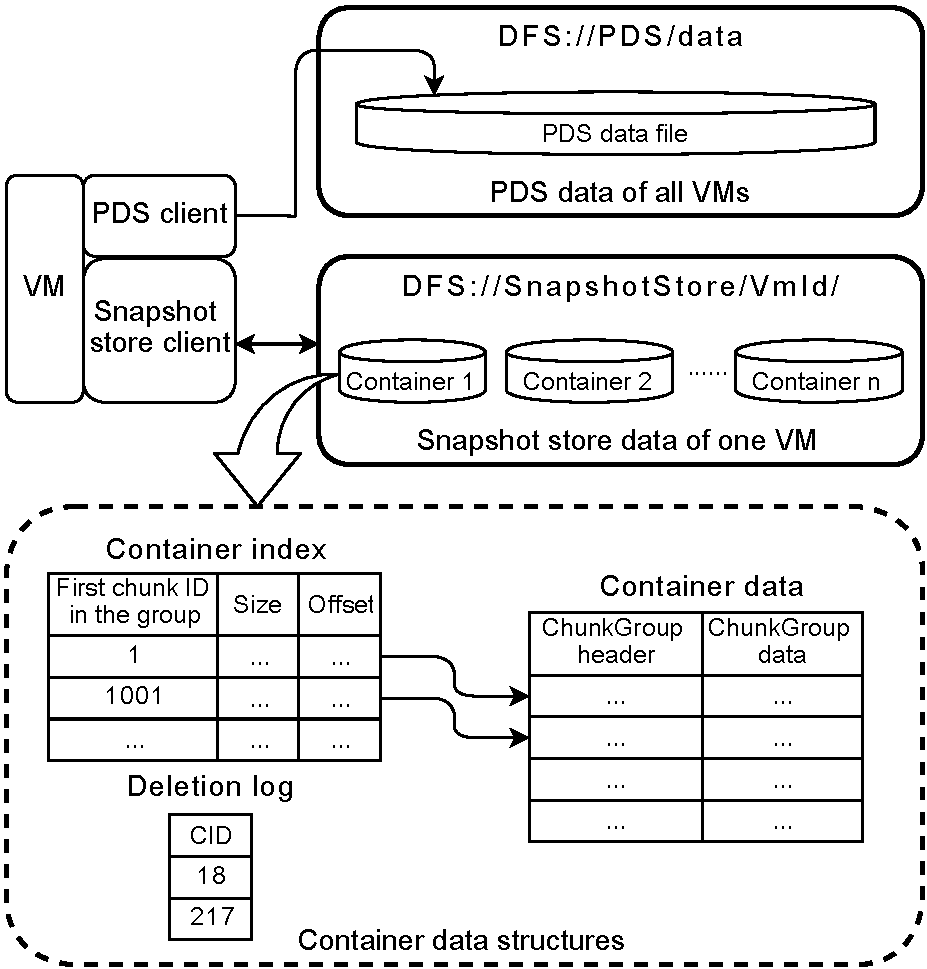
\includegraphics[width=2.75in]{images/sstore_arch}
  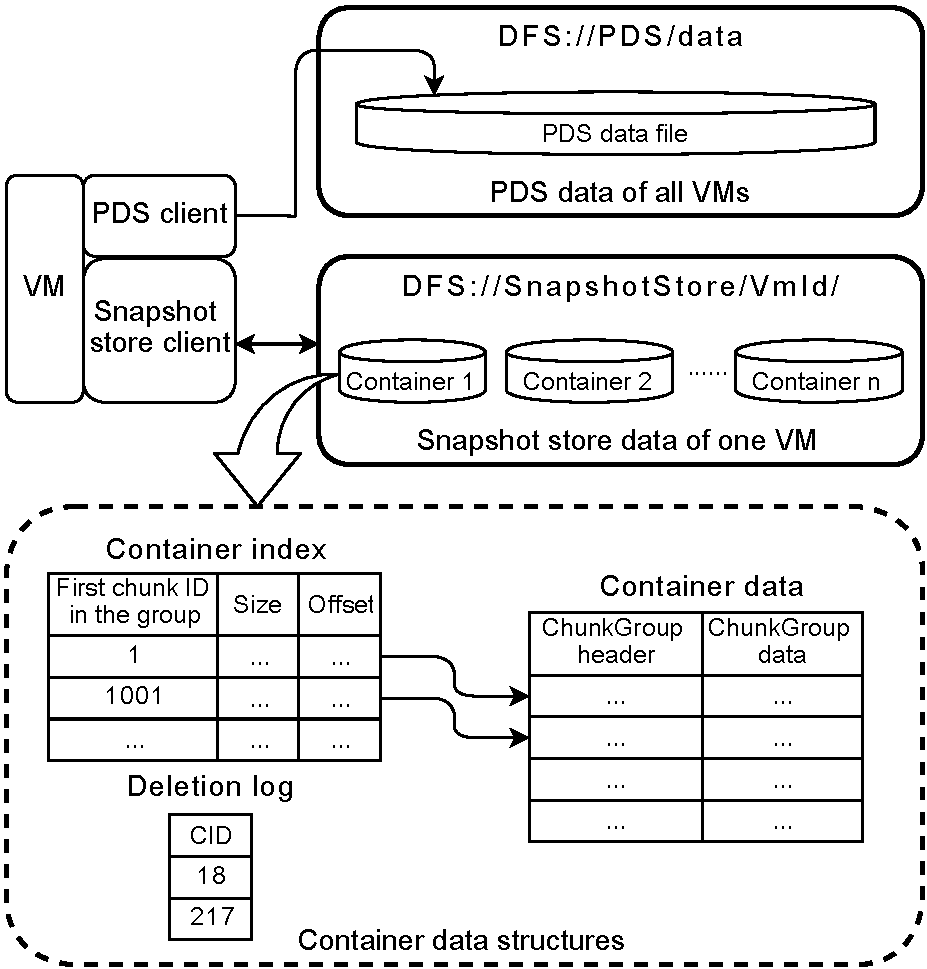
\includegraphics[width=2.2in]{images/sstore_arch}
  \caption{VM snapshot store data structures}
  \label{fig:as_arch}
\end{figure}

We use the QFS distributed file system to hold snapshot backups.
Following the VM-centric idea for the purpose of fault isolation,
each VM has its own snapshot store, containing new data chunks which are considered
to be non-duplicates.
As shown in Figure~\ref{fig:as_arch}, we explain the data structure of the snapshot stores as follows.
%\begin{itemize}
%\item
There is an independent store containing all PDS chunks shared among different VMs as
a single file.
%All PDS chunks are stored in one PDS file. 
Each reference to a PDS data chunk in the PDS index is the offset within the PDS file.
%There is an option to use a data structure similar to the non-PDS store. We opt
%for the simpler format because
Additional compression is not applied because 
for the data sets we have tested, we only observed limited spatial locality 
among popular data chunks. On average the number of consecutive PDS index hits is lower than 7,
thus it is not very effective to group a large number of chunks as a compression and data fetch unit. 
For the same reason, we decide not to take the sampled index approach~\cite{Guo2011} 
for detecting duplicates from PDS as limited spatial locality is not sufficient to enable
effective prefetching for sampled indexing.

PDS data are re-calculated periodically, but 
the total data size is small.  When
a new PDS data  set is computed, the in-memory PDS index is replaced, but 
the PDS file on the disk appends the  new PDS data identified and the growth of this file is very slow. 
The old data are not removed because they can still be referenced by the existing snapshots. 
A periodic cleanup is conducted  to remove unused PDS chunks (e.g. every few months). 

%\end{itemize}

For non PDS data, the snapshot store of a VM is  divided into a set of containers and 
each container is approximately 1GB. 
The reason for dividing the snapshot store into containers is to simplify the compaction process
conducted periodically. As discussed later, data chunks are deleted from old snapshots
and chunks without any reference from other snapshots can be removed by this compaction process.
By limiting the size of a container, we can effectively control the length of each round of compaction.
The compaction  routine can work on one container at a time and move the in-use data chunks to another container. 

Each non-PDS data container is further divided into a set of chunk data groups. Each chunk group is composed of
a set of data chunks and is the basic unit in data access and retrieval. 
In writing a chunk during backup, the system accumulates data chunks and stores the entire
group as a unit after compression. This  compression can reduce data by several times  in our tested data.
When accessing a particular chunk, its chunk group is retrieved from the storage
and decompressed. Given the high spatial locality and usefulness of prefetching  in 
snapshot chunk accessing~\cite{Guo2011,foundation08},
retrieval of  a data chunk  group naturally works well with prefetching. 
A  typical chunk group contains 1000 chunks in our experiment.
% with an average size of 200-600 chunks.

%\item
Each non-PDS data container is represented by three files in the DFS:
1) the container data file holds the actual content, 
2) the container index file is responsible for translating a data reference
into its location within a container, and 
3) a chunk deletion log file records all the deletion requests within  the container.

%\item
A non-PDS data chunk reference stored in the index of snapshot recipes
is composed of two parts: a container ID with 2 bytes and a local chunk ID with 6 bytes.
Each container maintains a local  chunk counter and assigns the current number 
as a chunk ID  when  a new chunk is added to this  container. 
Since data chunks are always appended to a snapshot store during backup, 
local chunk IDs are monotonically increasing.
When a chunk is to be accessed, the segment recipe contains a reference pointing to  a data chunk, which is used to lookup up the chunk data as described shortly.

%\item


Three API calls are supported for data backup:
%\begin{itemize}

%\item
\noindent\textbf{Append()}. 
For PDS data, the chunk is appended to the end of the PDS file and the offset is returned as the  reference.
Note that PDS append may only be used during PDS recalculation.
For non-PDS data, this call places a chunk into 
the snapshot store and returns a reference to be stored in 
the recipe metadata of a snapshot. 
The write requests to append data chunks to a VM store are accumulated at the client side. 
When the number of write requests reaches a fixed group size, the snapshot store client compresses
the accumulated   chunk group, adds a chunk group index  to the beginning of the group, and then
appends the header and data  to the corresponding VM file.
A new container  index entry is also created for each chunk group and is written to the corresponding
container index file.

%\item
\noindent\textbf{Get()}.
The fetch operation for the PDS data chunk is straightforward since each reference contains 
the file offset, and the size of a PDS chunk is available from a segment recipe.
We also maintain a small data cache for the PDS data service to speedup common data fetching.

To read a non-PDS chunk using its reference with container ID and local chunk ID,  the snapshot store client first loads the
corresponding VM's container index file specified by the container ID, then searches the chunk
groups  using their  chunk ID coverage.
After that, it reads the identified chunk group from DFS, decompresses it, and seeks to the exact chunk data 
specified by the chunk ID. 
Finally, the client updates its internal chunk data cache with the newly loaded content to 
anticipate future sequential reads.

%\item
\noindent\textbf{Delete()}.
Chunk deletion occurs when a snapshot expires or gets deleted explicitly by a user (the overall deletion strategy was discussed in detail in Section~\ref{sect:delete}).
When deletion requests are issued for a specific container,
those requests are simply recorded into the  container's deletion log initially and thus  a lazy
deletion strategy is exercised.
Once local chunk IDs appear in
the deletion log, they will not be referenced by any future snapshot and can be safely deleted when needed. 
This is ensured because we only dedup against the direct parent of a snapshot, so the deleted snapshot's blocks
will only be used if they also exist in other snapshots.
Periodically, the snapshot  store identifies those containers with an excessive
number of deletion requests to  compact and  reclaim the corresponding disk space. 
During compaction, the snapshot store creates a new container (with the same container ID) to replace the 
existing one. This is done by sequentially scanning the old container, copying all the chunks that are not 
found in the deletion log to the new container, and creating new chunk groups and indices. 
Every local chunk ID however is directly copied rather than re-generated. This
process leaves holes in the chunk ID values, but preserves the order and IDs of chunks.
As a result, all data references stored 
in recipes are permanent and stable, and the data reading process
is as efficient as before. Maintaining the stability of chunk IDs also ensures that recipes do not
depend directly on physical storage locations, which simplifies data migration.
%\end{itemize}



\section{Evaluation}
\label{sect:evaluation}
We have implemented and evaluated a prototype of our VC scheme on a Linux cluster of machines with
8-core 3.1Ghz AMD FX-8120 and 16 GB RAM. 
Our implementation is based on Alibaba cloud platform~\cite{Aliyun,WeiZhangIEEE}
and the underlying DFS uses  QFS with default replication degree 3 while the PDS replication degree is 6.
Our evaluation objective is to
study the benefit in fault tolerance and   deduplication efficiency of VC,  
and assess its backup throughput and  resource usage. 

We will compare VC with a VO approach  using stateless routing with binning (SRB) 
based on~\cite{Dong2011,extreme_binning09}.
SRB executes a distributed deduplication by routing a data chunk to one of cluster machines~\cite{Dong2011}
using  a min-hash function discussed in \cite{extreme_binning09}. Once a data chunk is routed to
a machine, the chunk is compared with the fingerprint index within this machine locally. 

\subsection{Settings}
We have performed a trace-driven study using a production dataset~\cite{WeiZhangIEEE} from 
Alibaba Aliyun's cloud platform with about 100 machines. 
Each machine hosts up to 25 VMs and each VM keeps 10 automatically-generated snapshots in the storage system while
a user may instruct extra snapshots to be saved.
The VMs of the sampled data set use popular operating systems such as 
Debian, Ubuntu, Redhat, CentOS, win2008 and win2003. 
%The backup of VM snapshots is required to complete within few  hours every night.
Based on our study of production  data,  each VM has about 40GB of storage  data  on average
including OS and user data disk.
%All data are divided into 2 MB fix-sized segments and 
The fingerprint for variable-sized chunks is computed using their SHA-1 hash~\cite{similar94,rabin81}. 
%Each segment is divided into 
%variable-sized content chunks with an average size of 4KB.
%Popularity of data blocks are collected through global counting and 
%and top popular ones ($\delta=2\%$)  are  kept in the PDS, as discussed in Section~\ref{sect:store}.

\subsection{Fault Isolation and Snapshot Availability}

 Table~\ref{tab:vm-availability} shows the availability of VM snapshots when 
there are up to 20 machine nodes failed in a 100-node cluster and  a 1000-node cluster. 
%Two VC curves use $V_c=1250$ and $V_c=2500$ representing the average number of VMs that share a PDS file system block. 
%We have assumed a worst-case scenario that  a PDS block is shared by every VM. 
%($V_c=p*V$), which is to be expected when PDS
%blocks are sorted by hash, as their order is randomized.
%$V_c=2500$ represents  the absolute worst case for 2500 VMs. 
%The VO curve has  $V_o=6.3$ which is the average number of VMs that share a file system block in our smaller dataset.
%To get this number, we perform perfect deduplication over 105 VMs, append unique chunks to a DFS file and
%count the number of dependencies from a file system block to VM.
%In the scenario of having 2500 VMs, this number can only increase, thus this number represents the best
%case for VO approach. 
%Our results show that the VC approach even with $V_c=2500$ has a higher availability than VO.
%For example, with 10 machines failed, VO with 98.5\% availability would lose snapshots of 37 VMs 
%while VC with 99.9\% loses snapshots of 2.5 VMs.
%The key reason is that  $N_1 +N_2 < N_o$, caused by the fact that the VM-centric approach localizes deduplication
%and packs  data blocks for one VM as much as possible.  The extra replication
%for PDS blocks also significantly increases the snapshot availability even when
%a PDS file block is shared by every VM.
%=======
%Figure~\ref{tab:vm-availability} shows the availability of VM snapshots
%as storage nodes fail. 
%We assume a random distirbution of 64MB file system
%blocks (FSBs). where FSBs are not randomly distributed availability might
%be improved by limiting the number of storage nodes a particualr VM depends
%on but we take the conservative approach. We compare VO, the expected case for
%VC ($V_c=p*V/2$), and the worst case for VC ($V_c=p*V/2$). We set $V_o=6.3$
%based on measured values in our dataset.
%To obtain VO sharing of file blocks, we perform perfect deduplication over 105 VMs, 
%append unique chunks to a DFS file and
%count the number of dependencies from a file system block to VM.
%In the case of having 2500 or even 25000 VMs, this number can only increase, thus this number represents the best
%case for VO approach. 
Our results show that VC has a significantly  higher availability than VO as the number of
failed machines increases.
%Our VM-centric approach shows significant improvements
%in VM availability.
For example, with 3/100 machines failed and 25 VMs per machine, VO with 69.5\% availability could lose data in 763 VMs 
while VC with 99.7\% loses data for 8 VMs.
The key reason is that for most data in VC, only a single VM can be affected by
the loss of a single file block. Since most blocks contain chunks for a single
VM, VMs can depend on a smaller number of blocks, while in VO, the loss of a
single block tends to affect many VMs.
% because our VM-centric approach
%localizes deduplication.  

Although the loss of a PDS block affects many VMs,
by increasing replication for those blocks we minimize the effect on VM
snapshot availability, and this is one of the key contributions of our
approach, the clear separation of highly popular data from less popular data.
%By having extra replicas for the PDS data, we reduce the failure rate of PDS
%FSBs enough that the failure rate for the VM approaches the failure rate of the
%Non-PDS blocks. This minimizes the drop in availability between the expected
%and worst case for VC.
%
%One of the advantages of VC is that there is a division between
%popular and non-popular data to facilitate improved reliability. 
Figure~\ref{fig:pds-replication} shows
the impact of increasing PDS data replication. 
While the impact on storage cost is small (because we have separated out only
the most popular blocks),
a replication degree of 6  has a significant improvement over 4. The
availability is very similar
for $r_c=6$ and $r_c=9$, and beyond $r_c=6$ improvements are minimal.
 
%This is because, as described before, the availability of the VM approaches the
%availiability of the Non-PDS data as the failure rate of PDS data gets very small.

\comments{
\begin{figure}[ht]
    \centering
    \begin{subfigure}%{.5\textwidth}
      \centering
      %\includegraphics[scale=.45,natwidth=511,natheight=276]{vo_links}
            \begin{tikzpicture}
                    \begin{axis}[
                    tick label style={font=\scriptsize},
                    tick style=thin,
                    width=0.5\linewidth,
                    title={\small $p=100$},
                    cycle list={
                        {blue,thin,solid,mark=none},
                        {red,thin,densely dashed,mark=none},
                        {red,thin,densely dotted,mark=none}
                    },
                    xlabel={\tiny Failed nodes},
                    ylabel={\tiny Snapshot Availability (\%)},
                    %extra y ticks={99.9}, %if important numbers are missing
                    mark options=solid,
                    legend columns=-1,
                    legend style={
                        font=\small\sffamily,
                        cells={anchor=west}, %legend entry alignment
                        legend pos=south west %legend position
                    },
                    legend to name=legend:vm-availability,
                    %reverse legend,
                    ]
                    \addplot table[x=NodesFailed,y=VO]{figures/node_failures_100.txt};
                    \addlegendentry{VO}
                    \addplot table[x=NodesFailed,y=VC3]{figures/node_failures_100.txt};
                    \addlegendentry{VC}
                    %\addplot table[x=NodesFailed,y=VCOpt1]{figures/node_failures_100.txt};
                    %\addlegendentry{VC (CDS ordering)}
                    \end{axis}
            \end{tikzpicture}
      %\caption{100 machine cluster.}
      \label{fig:vm-availability-100}
    \end{subfigure}%
    \begin{subfigure}%{.5\textwidth}
  \centering
  %\includegraphics[scale=.45,natwidth=511,natheight=276]{vo_links}
	\begin{tikzpicture}
            %the expressions in this plot are simply to trick pgfplots into not expanding the y range, and don't actually change the data
            % expression used: (99.999+((y-99.999)*1000)/1000)
            \pgfplotsset{/pgf/number format/.cd,
                fixed,precision=4}
		\begin{axis}[
                    width=0.5\linewidth,
                    tick label style={font=\scriptsize},
                    tick style=thin,
		title={\small $p=1000$},
                %ymin=099.9991,
                %ymax=100.0002,
                %ytick=data,
                %yticklabels from table={figures/vm_availability_1000.txt}{[index]1},
                yticklabel={%this is a hack to get around the small yrange
                    \pgfmathfloatparse{99.999+\tick/1000}
                    \pgfmathprintnumber{\pgfmathresult}
                },
                cycle list={
                    {blue,thin,solid,mark=none},
                    {red,thin,densely dashed,mark=none},
                    {red,thin,densely dotted,mark=none}
                },
		xlabel={\tiny Failed nodes},
		ylabel={\tiny Snapshot Availability (\%)},
		%extra y ticks={99.99}, %if important numbers are missing
                mark options=solid,
                legend style={
                    cells={anchor=west}, %legend entry alignment
                    legend pos=south west %legend position
                },
                %reverse legend,
		]
                %\addplot table[x=NodesFailed,y=VO1]{figures/vm_availability_1000.txt};
                \addplot table[x=NodesFailed,y expr=(\thisrow{VO}-99.999)*1000]{figures/node_failures_1000.txt};
                %\addlegendentry{$VO\,6.3$ (optimistic)}
                %\addplot table[x=NodesFailed,y=VC1]{figures/vm_availability_1000.txt};
                \addplot table[x=NodesFailed,y expr=(\thisrow{VC3}-99.999)*1000]{figures/node_failures_1000.txt};
                %\addlegendentry{$VC\,1250$ (estimated)}
                %\addplot table[x=NodesFailed,y=VC2]{figures/vm_availability_1000.txt};
                \addplot table[x=NodesFailed,y expr=(\thisrow{VCWC1}-99.999)*1000]{figures/node_failures_1000.txt};
                %\addlegendentry{$VC\,2500000$ (worst-case)}
                %\addplot table[x=NodesFailed,y=VO2]{figures/vm_availability.txt};
                %\addlegendentry{$VO\,20$ (optimistic)}
		\end{axis}
	\end{tikzpicture}
        %\caption{1000 machine cluster.}
  \label{fig:vm-availability-1000}
\end{subfigure}
    \pgfplotslegendfromname{legend:vm-availability}
      \caption{Availability of VM snapshots for VO and VC when failed machines vary
from 1 to 40.  Non-PDS replication is fixed
at 3 and PDS replication is 6 \emph{THIS PLOT IS BEING REPLACED BY A TABLE} 
      }
      \label{fig:vm-availability}
   
 
\end{figure}
}
\begin{table}
  \centering
    \footnotesize
    \tabcolsep=0.11cm
    \pgfplotstabletypeset[
        comment chars=!,%use ! before a row in the data table to exclude it
        columns={NodesFailed,VO100,VC100,VO1000,VC1000},
        columns/NodesFailed/.style={
            column name={\multirow{3}{*}{Failures ($d$)}}
        },
        columns/VO100/.style={
            column name={
                \multicolumn{4}{c|}{VM Snapshot Availability(\%)}\\&
                \multicolumn{2}{c|}{$p=100$}&\multicolumn{2}{c|}{$p=1000$}\\&
            VO},
            fixed, precision=6
        },
        columns/VC100/.style={
            column name={VC},
            fixed, precision=6},
        columns/VO1000/.style={
            column name={VO},
            fixed, precision=6},
        columns/VC1000/.style={
            column name={VC},
            fixed, precision=6},
        every head row/.style={
            before row={\hline},
            after row={\hline},
        },
        every last row/.style={after row=\hline},
        column type/.add={}{|},
        every first column/.style={column type/.add={|}{}},
        %the below rows can be used to extract rows 3,5,10,20 from rows 0-40
        %skip rows between index={0}{3},
        %skip rows between index={4}{5},
        %skip rows between index={6}{10},
        %skip rows between index={11}{20},
        %skip rows between index={21}{41}
    ]{figures/availability_table.txt}
    \caption{Availability of VM snapshots for VO and VC ($r_c=6$).}
    \label{tab:vm-availability}
\end{table}

\begin{figure}[htb]
  \centering
	\begin{tikzpicture}
		\begin{axis}[
                        width=\linewidth,
                        height=0.6\linewidth,
		%title={PDS Replication affect on availability},
		xlabel={Failed storage nodes},
		ylabel={VM Snapshot Availability (\%)},
                xmin=0,
                xmax=10,
		%extra y ticks={99.9}, %if important numbers are missing
                mark options=solid,
                legend style={
                    cells={anchor=west}, %legend entry alignment
                    legend pos=south west %legend position
                },
                reverse legend,
		]
                \addplot+[dashed] table[x=NodesFailed,y=VO]{figures/node_failures_100.txt};
                \addplot table[x=NodesFailed,y=VC1]{figures/node_failures_100.txt};
                \addplot table[x=NodesFailed,y=VC2]{figures/node_failures_100.txt};
                \addplot table[x=NodesFailed,y=VC3]{figures/node_failures_100.txt};
                \addplot table[x=NodesFailed,y=VC4]{figures/node_failures_100.txt};
                \legend{
                    VO,
                    $r_c=4$,
                    $r_c=5$,
                    $r_c=6$,
                    $r_c=9$
                }
		\end{axis}
	\end{tikzpicture}
  \caption{Availability of VM snapshots in VC with different PDS replication degrees}
  \label{fig:pds-replication}
\end{figure}

\comments{
\begin{figure}[htb]
  \centering
	\begin{tikzpicture}
		\begin{axis}[
                        width=\linewidth,
                        height=0.6\linewidth,
		%title={PDS Replication affect on availability},
		xlabel={Failed storage nodes},
		ylabel={VM Snapshot Availability (\%)},
                xmin=0,
                xmax=20,
		%extra y ticks={99.9}, %if important numbers are missing
                mark options=solid,
                legend style={
                    cells={anchor=west}, %legend entry alignment
                    legend pos=south west %legend position
                },
                reverse legend,
		]
                %\addplot+[dashed] table[x=NodesFailed,y=VO]{figures/node_failures_100.txt};
                %\addplot table[x=NodesFailed,y=VC1]{figures/node_failures_100.txt};
                \addplot table[x=NodesFailed,y=VC2]{figures/node_failures_100.txt};
                \addplot table[x=NodesFailed,y=VC3]{figures/node_failures_100.txt};
                \addplot table[x=NodesFailed,y=VC4]{figures/node_failures_100.txt};
                \legend{
                    %VO,
                    %$r_c=4$,
                    $r_c=5$,
                    $r_c=6$,
                    $r_c=9$
                }
		\end{axis}
	\end{tikzpicture}
  \caption{Availability of VM snapshots in VC with different PDS replication degrees \todo{decide which one}}
  \label{fig:pds-replication-old}
\end{figure}

}

\subsection{Deduplication Efficiency}
\label{sect:evaldedup}

\comments{
%this version combines the old and the minhash alg. to compare against srb
\begin{figure}[ht]
  \centering
    \begin{tikzpicture}
            \begin{axis}[
            %title={Ex-Binning Efficiency},
            width=\linewidth,
            height=0.75\linewidth,
            cycle list={%
                {blue,solid,mark=square*},
                {blue,solid,mark=triangle*,mark size=1.5},
                {blue,solid,mark=diamond*,mark size=1.5},
                %{blue,solid,mark=pentagon*,mark size=1.4},
                {red,draw=red,dotted,mark=square},
                %{red,densely dotted,mark=triangle,mark size=1.5},
                %{red,densely dotted,mark=diamond,mark size=1.5},
                {brown,dashed,mark=*},
                %{red,densely dotted,mark=o},
                %{red,densely dotted,mark=pentagon,mark size=1.4},
            },
            mark repeat={10},
            xlabel={Number of VMs added},
            ylabel={Dedup. Efficiency (\%)},
            xmin=0,
            ymin=85,
            ymax=100,
            %extra y ticks={4.5,5.5,6.5} %to add extra ticks
            mark options=solid,
            legend pos=south west,
            legend columns=2,
            legend style={
                font={\tiny\sffamily},
                nodes={right}
                %at={(0.5,-0.2)},
                %anchor=north
            },
            ]
            \addplot table[x=VMs,y=MHcds4] {figures/exbin_efficiency_comparison2.txt};
            \addplot table[x=VMs,y=MHcds2] {figures/exbin_efficiency_comparison2.txt};
            %\addplot table[x=VMs,y=MHcds1] {figures/exbin_efficiency_comparison2.txt};
            \addplot table[x=VMs,y=MHNocds] {figures/exbin_efficiency_comparison2.txt};
            %\addplot table[x=VMs,y=cds4] {figures/exbin_efficiency_comparison2.txt};
            \addplot table[x=VMs,y=cds2] {figures/exbin_efficiency_comparison2.txt};
            %\addplot table[x=VMs,y=cds1] {figures/exbin_efficiency_comparison2.txt};
            \addplot table[x=VMs,y=exbin] {figures/exbin_efficiency_comparison2.txt};
            \legend{VC( $\sigma=4\%$),
                VC($\sigma=2\%$),
                %VC MH($\sigma=1\%$),
                VC(No PDS),
                %VC($\sigma=4\%$),
                VC($\sigma=2\%$\, No similarity guidance),
                %VC($\sigma=1\%$),
                SRB
            };
            \end{axis}
    \end{tikzpicture}
    \caption{Deduplication efficiency of VC and SRB.}
  \label{fig:exbin-efficiency-graph2}
\end{figure}

}

\begin{figure}[]
    \centering
    \begin{tikzpicture}
        \begin{axis}[
                width=\linewidth,
                height=0.6\linewidth,
                ybar,
                bar width=0.5cm,
                ymax=98.7,
                enlarge x limits=0.15,
                style=thin,
                ylabel={Dedup. Efficiency (\%)},
                ytick={93,94,95,96,97,98},
                xtick=\empty,
                ymajorgrids,
                grid style=densely dotted,
                %symbolic x coords={VC-No PDS, VC-2\%PDS w/o similarity, VC-2\%PDS, VC-4\%PDS, SRB},
                %symbolic x coords={VC0, VC2N, VC2, VC4, SRB},
                %xticklabels from table={figures/efficiency_comparison_bars.txt}{alg}
                nodes near coords,
                every node near coord/.append style={
                    anchor=-145+\coordindex*10
                }
            ]
            %\addplot[fill=blue] coordinates {(VC0,93.02) (VC2N,94.31) (VC2,96.01) (VC4,96.58) (SRB,97.86)};
            %\addplot[fill=blue] coordinates { (VC-No PDS,93.02) (VC-2\%PDS w/o similarity,94.31) (VC-2\%PDS,96.01) (VC-4\%PDS,96.58) (SRB,97.86) };
            \addplot [%
                point meta=explicit symbolic,
                fill=blue
            ] table [x expr=\coordindex, y=efficiency,meta=alg] {figures/efficiency_comparison_bars.txt};
        \end{axis}
    \end{tikzpicture}
    \caption{Efficiency Comparison between different VC settings and SRB}
    \label{fig:efficiency-comparison}
\end{figure}

Figure~\ref{fig:efficiency-comparison} shows the deduplication efficiency for SRB and VC using different settings,
% <<<<<<< HEAD
% Our deduplication efficiency is defined as the percent of duplicate chunks
% which are detected and deduplicated, so only global perfect deduplication can have 100\% efficiency.
% The figure also compares several PDS sizes chosen for VC. ``$\sigma=2\%$'' 
% is defined in Table~\ref{tab:symbol}. 
% =======
that is the percent of duplicate chunks
which are detected and removed.
% so only global perfect deduplication can have 100\% efficiency.
% We also compare several PDS sizes chosen for VC.
%(see Table~\ref{tab:symbol} for definition of ``$\sigma=2\%$'')
%we allocate the space of distributed shared memory  to accommodate 2\%
%of data chunks shared among VMs, as defined in 
With $\sigma=2\%$, memory usage for PDS index lookup per machine is about 100MB per machine
and  the deduplication efficiency can reach over 96\%.
When $\sigma=4\%$, the deduplication efficiency can reach 96.6\% while space consumption increases to 200MB per machine. 
%and  the deduplication efficiency can reach 96.489\%.
%When $\sigma=4\%$, the deduplication efficiency can reach 97.027\% while space consumption increases to 200MB per machine. 
The loss of efficiency in VC is caused by the restriction of the physical memory available
in the cluster for fast in-memory PDS index lookup. 
%In the extreme case if we put all the fingerprint into PDS 
%index ($\sigma=100\%$) then VC will have 100\% efficiency.
SRB can deliver up to 97.86\% deduplication efficiency, which is slightly better than VC.
Thus this represents a tradeoff that VC provides better fault tolerance and fast approximate deletion
with a slight reduction in deduplication efficiency.

% SRB can deliver up to 97.935\% deduplication efficiency which is slightly better than VC.
% Thus this represents a tradeoff: VC provides better fault tolerance and fast
% approximate deletion with competitive (but slightly lower) deduplication
% efficiency.
% >>>>>>> 4dcd68612b052c0f890ed30361a9ed03771b5df1
%its loss of efficiency is caused by the routing of data chunks which restricts the search scope
%of duplicate detection.
%SRB provides slightly better deduplication efficiency than our VC approach, which we accept
%because we are rewarded by architecture-wise benefits such as fault-tolerance and fast 
%Though not our primary goal, this result does show that VC can remove competitive amount of duplicates.

Figure~\ref{fig:efficiency-comparison} also shows the efficiency of VC without local similarity search.
%There is a big efficiency drop in this curve when the number of VMs is about 30.
The reason similarity search provides such an improvement is that
%Without this (i.e. when we only 
there are VMs in which
data  segments are moved to another location on disk, for example when a file is rewritten
rather than modified in place,  
and a dirty-bit or offset-only based detection would not be able to detect such a movement.
We have found that in
approximately 1/3 of the VMs in our dataset this movement happens frequently.
In general, adding local similarity-guided search increases deduplication efficiency from 94\% to over 96\%.
That is one significant improvement compared to the work in ~\cite{WeiZhangIEEE}
which uses the parent segment at the same offset to detect duplicates instead of similarity-guided search.
% In general, our experiments show that
% dirty-bit detection at the segment level can reduce the data size to about 24.14\% of original data, 
% which leads about a 75.86\% reduction.
% Similarity-guided local search can further reduce the data size
% to about 12.05\% of original size, namely it delivers an additional 12.09\% reduction.
% The PDS-based global duplicate detection with $\sigma=2\% $
% can reduce the size further to 8.6\% of original size, namely it 
% delivers an additional 3.45\% reduction.

In general, our experiments show that
dirty-bit detection at the segment level can reduce the data size to about 24.14\% of original data, 
which leads to about a 75.86\% reduction.
Similarity-guided local search can further reduce the data size
to about 12.05\% of original, namely it delivers a 50.08\% reduction to the dirty segments.
The popularity-guided global deduplication with $\sigma=2\% $
can reduce the data further to 8.6\% of its original size, so
it provides additional 28.63\% reduction to the remaining data.

%Figure~\ref{fig:exbin-efficiency-graph2} also shows the benefits of our minhash
%similar segment search in the parent snapshot. 

\subsection{Resource Usage and Processing Time}

\comments{
\begin{table}
    \begin{tabular}{|c|c|}
    \hline
    PDS replication degree & Disk usage per machine  \\ \hline
    3                      & 3065GB             \\ \hline
    4                      & 3072GB             \\ \hline
    5                      & 3079GB             \\ \hline
    6                      & 3086GB             \\ \hline
    7                      & 3093GB             \\ \hline
    \end{tabular}
\caption{Storage space cost per machine for DFS under different PDS replication degree}
\label{tab:replication_cost}
\end{table}
}

{\bf Storage cost of replication.} 
%Table ~\ref{tab:replication_cost} shows the total storage space required by 
%VC as the PDS replication degree changes while non-PDS replication degree is fixed as 3. 
When the replication degree of both PDS and non-PDS data is 3, 
the total storage  for all VM snapshots in each physical machine takes about 3.065TB on average before compression
and 0.75TB after compression.  Allocating  one extra  copy for PDS data only adds  7GB in total per machine.
Thus PDS replication degree 6 only increases the total space by 0.685\% while PDS replication degree 9 adds 1.37\% 
space overhead, which is still small.
%The increase in storage cost is minimal because the PDS makes up a 
%small percent of the total storage space, while increasing replication degree has a  more significant benefit for
%availability as shown in Figure~\ref{fig:pds-replication}.

\begin{table}
    \begin{tabular}{|c|c|c|c|c|c|}
    \hline
    Tasks & CPU & Mem &Read &  Write  & Time  \\ 
    & & (MB)          &(MB/s) &  (MB/s) & (hrs) \\ \hline
%    1     & 19\% & 118.1 & 50MB/s 8.37 & 1.314\\ \hline
    1     & 19\% & 118 & 50 & 16.4 & 1.31\\ \hline
%    2     & 35\% & 131.8 & 9.0 & 1.226\\ \hline
    2     & 35\% & 132 &50  & 17.6 & 1.23\\ \hline
    %4     & 63\% & 154.1 & 9.3 & 1.179\\ \hline
    4     & 63\% & 154&50   & 18.3 & 1.18\\ \hline
    6     & 77\% & 171.9 & 50 &  18.8 & 1.162\\ \hline
%    8     & 82\% & 90.5 & 89.2 & \\ \hline
%    10                      & 85\% & 97.2   & 90.4 \\ \hline
%    12                      & 91\% & 95.6    & 91.5 \\ \hline
    \end{tabular}
\caption{Resource usage of concurrent backup tasks at each machine}
\label{tab:resource_usage}
\end{table}

{\bf Memory and disk bandwidth usage with multi-VM processing}. 
We have further studied the memory and disk bandwidth usage 
when running concurrent VM snapshot backup on each machine with $\sigma=2\%$. 
Table ~\ref{tab:resource_usage} gives the resource usage  when
running 1 or multiple  VM backup tasks at the same time on each physical machine. 
``CPU'' column is the percentage of a single core used. 
``Mem'' column includes 100MB memory usage for PDS index and other space cost for executing deduplication tasks such as 
receipt metadata and cache. 
``Read'' column is controlled as 50MB/s bandwidth usage with I/O throttling so that other cloud services are not impacted too much.
The peak raw storage read performance is about 300MB/s and we only use 16.7\% with this collocation consideration.
``Write'' column is the I/O write usage of QFS and notice that each QFS write triggers disk writes in multiple machines due to
data replication.     50MB/s dirty segment read speed triggers about 16.4MB/s disk write for non duplicates with one backup task.
% [ NOT REASONABLE: Notice that memory and CPU used by PDS index and QFS are not included since they belong to 
% the cloud infrastructure services and are shared among many applications.]
%We see our hybrid deduplication scheme only occupies a small amount of system resources. 
%The  local deduplication only needs to keep the parent snapshot recipe and a few similar segment recipes in 
%memory during duplicate detection.

Table ~\ref{tab:resource_usage} shows that  a single backup task per node can complete the backup of the entire
VM cluster in about 1.31 hours. Since there are about 25 VMs per machine, we could execute
more tasks in parallel at each machine. But adding more backup concurrency does not shorten the overall time
significantly because of the controlled  disk read time.
%,  we can still process raw data at near 175 MB/s. If we consider the extreme case in which each machine has 25 VMs
%at 40GB size, our snapshot system can finish backing up all the VMs (1TB total) in 1.58 hours.

{\bf Processing Time breakdown}.
Figure~\ref{fig:vc_srb_combined} shows
the  average  processing  time of  a VM segment under VC and SRB. 
VC uses $\sigma=2\%$ and $4\%$.
It has a breakdown of processing time.
``Snapshot read/write'' includes snapshot reading and writing from disk, and 
updating of the metadata.
`` Network transfer" includes the cost of transferring raw and meta data from one machine to another during 
snapshot read and write.
``Index access/comparison'' is the disk, network and CPU time during fingerprint comparison.
This includes PDS data lookup for VC and index lookup from disk in VO after Bloom filter lookup.
For VC, the change of $\sigma$ does not significantly affect the overall backup speed as
PDS lookup takes only a small amount of time. The network transfer time for VC and SRB is about the same, because the 
amount of raw data they transfer is comparable.
SRB spends slightly more time for snapshot read/write because during each snapshot  backup, SRB involves many small bins,
 while VC only involves few containers with a bigger size. Thus, there are more opportunities for I/O aggregation in VC to reduce seek time.
SRB has a higher cost for index access and fingerprint comparison because most of  chunk fingerprints are routed
to remote machines for comparison while   VC handles most of chunk fingerprints locally. 

%on the index holding machine to access its index (often on the disk, supported by a Bloom filter) 
%and perform comparison.
%VC is faster in this regard because it conducts in-memory local search first and then
%accesses  the PDS on distributed shared memory, so most chunks can be dealt with locally.  
%SRB spends  slighter more time in  reading data and updates because it also updates the on-disk
%local meta data index in addition to partition indices.
%As a result Overall,  VC is faster than SRB, though data reading dominates the processing time for both algorithms.
%Figure~\ref{fig:vc_srb_combined} also reports the average backup time for a VM in VC when
%varying the PDS size.  It lists the time distribution for data reading,
%similarity-guided local search, global PDS lookup, and non-duplicate data writing. 
%While data reading dominates the backup process, PDS lookup spends about a similar amount
%of time as local search.

\begin{table}
  \centering
    \footnotesize
    %\tabcolsep=0.11cm
    \pgfplotstabletypeset[
        comment chars=!,%use ! before a row in the data table to exclude it
        col sep=tab,
        %columns={Algorithm,Snapshot Read/Write,Network Transfer,Index access and comparison},
        columns={Algorithm,ReadWrite,Network,Index},
        columns/Algorithm/.style={
            string type,
            column name={\multirow{2}{*}{Algorithm}}
        },
        columns/ReadWrite/.style={
            column name={
                \multicolumn{3}{c|}{Time Spent in Task (ms)}\\&
                Read/Write
            },
            multiply by={1000},
            %preproc cell content/.code={1#1 1},
            fixed, precision=3
        },
        columns/Network/.style={
            column name={Network},
            multiply by={1000},
            fixed, precision=3
        },
        columns/Index/.style={
            column name={Index Lookup},
            multiply by={1000},
            fixed, precision=3
        },
        every head row/.style={
            before row={\hline},
            after row={\hline},
        },
        every last row/.style={after row=\hline},
        column type/.add={}{|},
        every first column/.style={column type/.add={|}{}},
    ]{figures/vc_srb_combined_pgfplots.txt}
    \caption{Average time to backup a dirty VM segment under SRB and VC
        \todo{Decide between this and bar plot with the same caption}
    }
    \label{tab:vc_srb_combined}
\end{table}

\begin{figure}[htbp]
  \centering
  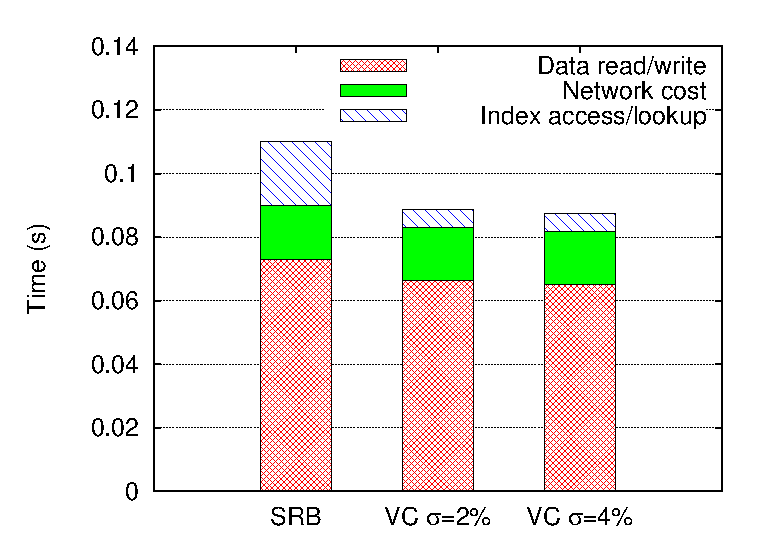
\epsfig{file=figures/vc_srb_combined, width=3in}
  \caption{Average time to backup a dirty VM segment under SRB and VC}
  \label{fig:vc_srb_combined}
\end{figure}

% \begin{figure}[htbp]
%   \centering
%   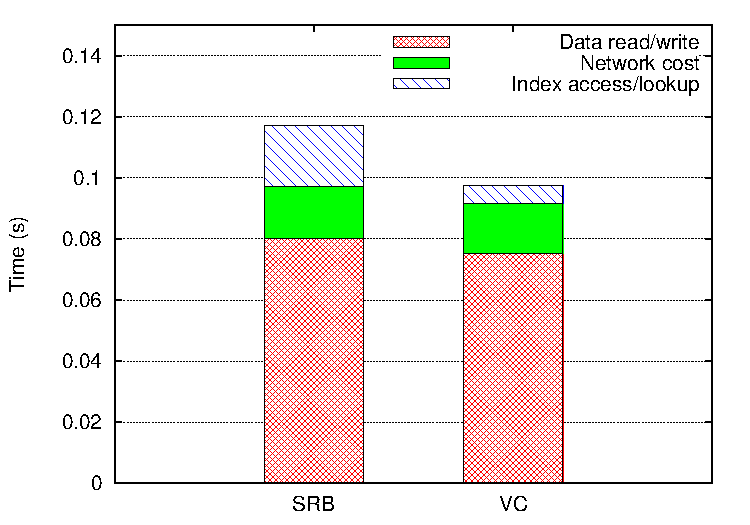
\epsfig{file=figures/srb_vs_vc, width=3in}
%   \caption{Time to backup a dirty VM segment under SRB and VC}
%   \label{fig:srb_vs_vc}
% \end{figure}


% \begin{figure}
%     \centering
%     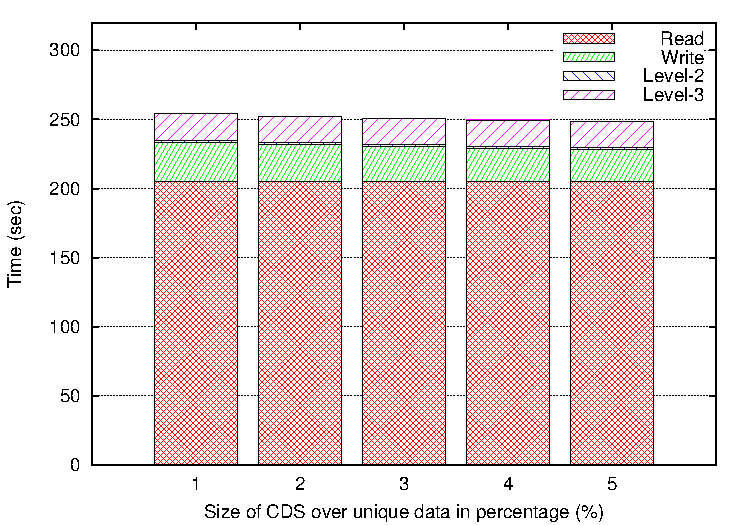
\includegraphics[width=3in]{figures/single_backup_time}
%     \caption{Average time to backup a VM in VC with varying PDS sizes}
%     \label{fig:single_vm_backup}
% \end{figure}


% \begin{table*}[t]
%     \centering
%     \begin{tabular}{c|ccc|ccc}
%     Num. of concurrent      & \multicolumn{3}{c|}{Throughput without}    & \multicolumn{3}{c}{Throughput with} \\
%     backup tasks            & \multicolumn{3}{c|}{I/O throttling (MB/s)} & \multicolumn{3}{c}{I/O throttling (MB/s)} \\ \cline{2-7}
%     per node                & Raw                                        & Snapshot Store & QFS  & Raw                                    & Snapshot Store & QFS  \\ \hline
%     1                       & 1369.6                                     & 148.0          & 18.0 & 171.3                                  & 18.5           & 2.26 \\
%     2                       & 2408.5                                     & 260.2          & 31.7 & 201.3                                  & 21.8           & 2.66 \\
%     4                       & 4101.8                                     & 443.3          & 54.1 & 217.8                                  & 23.5           & 2.87 \\
%     6                       & 5456.5                                     & 589.7          & 72.0 & 224.1                                  & 24.2           & 2.96 \\
%     \end{tabular}
% \caption{Throughput of software layers under different concurrency}
% \label{tab:throughput}
% \end{table*}
\begin{table}[htbp]
\begin{small}
    \centering
    \begin{tabular}{|c|ccc|}
\hline
    Concurrent      & \multicolumn{3}{c|}{Throughput without}    \\
    backup tasks            & \multicolumn{3}{c|}{I/O throttling (MB/s)} \\ \cline{2-4}
    per machine                & Backup                                     & Snapshot Store & QFS  \\ 
    		&                                      & (write) & (write)  \\ \hline
    1                       & 1369.6                                     & 148.0          & 35.3 \\
    2                       & 2408.5                                     & 260.2          & 61.7 \\
    4                       & 4101.8                                     & 443.3          & 103.1 \\
    6                       & 5456.5                                     & 589.7          & 143.8 \\ \hline
    \end{tabular}
\end{small}
\caption{Throughput of software layers per machine under different concurrency}
\label{tab:throughput}
\end{table}

{\bf Throughput of software layers.}
Table~\ref{tab:throughput} shows the  average throughput of software layer
when when I/O throttling is not applied to control the usage.
%machine when all machine nodes execute one or multiple MV backup tasks.
``Backup'' column is the throughput  of the backup service  per machine.
``Snapshot store" is the  write throughput of the snapshot store layer. The gap between this
column and  ``Backup" column is caused by significant data reduction by dirty bit and duplicate
detection. Only non-duplicate chunks trigger a snapshot store write.
``QFS'' column is the write request traffic to the underlying file system after compression.
For example, with 148MB/second write traffic to the snapshot store, QFS write traffic is about 35.3MB/second
after compression.  The underlying disk storage traffic will be three times greater with replication.
The result shows that the backup service can deliver up to 5.46GB/second without I/O restriction
per machine with 6 concurrent backup tasks. With a higher disk storage bandwidth available, the above backup
 throughput would be higher. 
%With 50MB/second controlled I/O bandwidth, each machine can deliver 171MB/second with 1 backup task and can complete the backup of 25 VMs per machine in less than 1.31 hours.
 
%To begin, on each node we write snapshots for 4 VMs concurrently, and gradually 
%increase number of VMs to 12 to saturate our system capability. 
%We observed 
%the per-node throughput peaked at 2700 MB/s when writing 10 VM snapshots in parallel, 
%which is far beyond our QFS file system capability. The reason behind it is our efficient
%deduplication architecture and compression which greatly reduce the amount of data that needs to be written to
%the file system. The main bottleneck here is that our QFS installation only
%manages one disk per node, which prevents it from fully utilizing the
%benefits of parallel disk access. We expect our architecture can
%perform even better in production clusters, which often have ten or more disks on each node.


% \begin{figure}
%     \centering
%     \subfigure[Backup throughput per node under controlled I/O bandwidth usage]
%     {
%         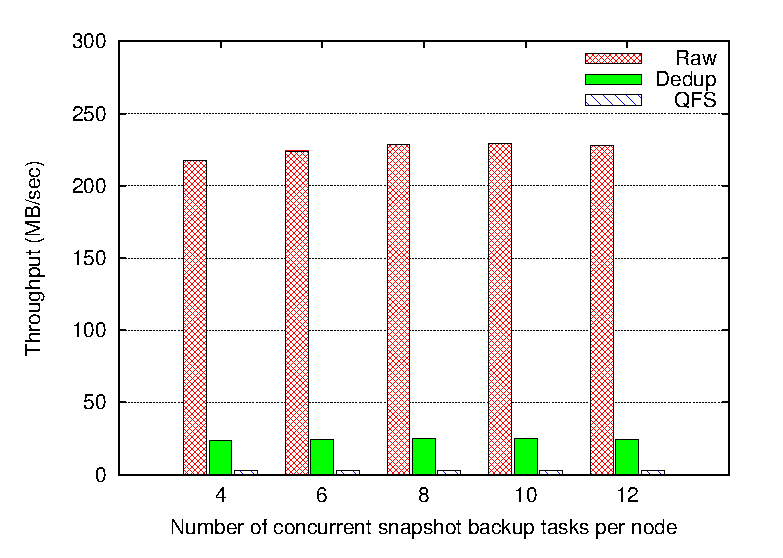
\includegraphics[width=3in]{figures/parallel_backup_with_read}
%         \label{fig:withread}
%     }
%     \\
%     \subfigure[Deduplication and storage system performance]
%     {
%         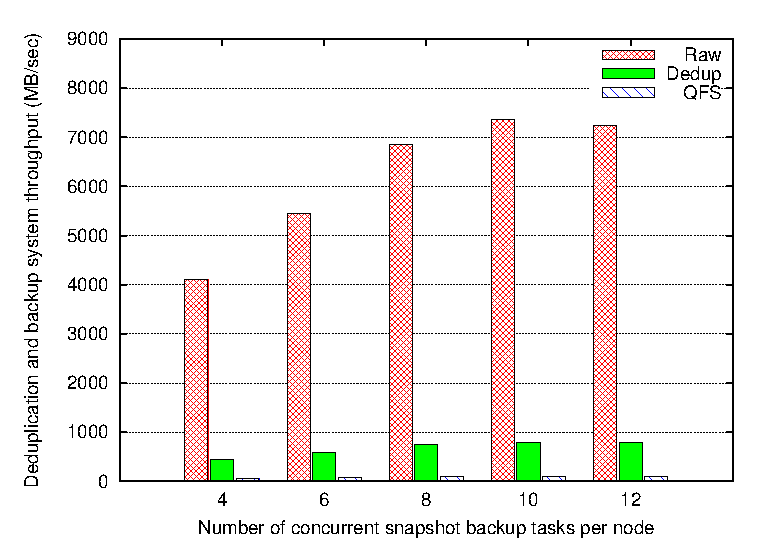
\includegraphics[width=3in]{figures/parallel_backup_no_read}
%         \label{fig:noread}
%     }
%     \caption{Throughput per-node with concurrent snapshot backup tasks}
%     \label{fig:parallel_backup}
% \end{figure}

 \subsection{Effectiveness of Approximate Deletion}

 \begin{figure}
     \centering
     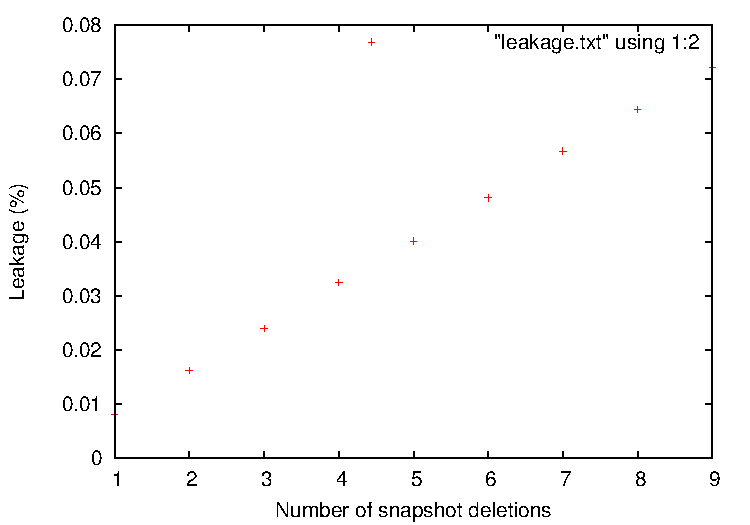
\includegraphics[width=3in]{figures/leakage}
     \caption{Accumulated storage leakage by approximate snapshot deletions ($\Delta u/u=0.025$)}
     \label{fig:leakage}
 \end{figure}

Figure~\ref{fig:leakage} shows the average accumulated storage leakage in terms of percentage of
storage space per VM caused  by approximate deletions.
We choose 35 VMs, first let all the VMs accumulate to 10 snapshots, then start to delete snapshots
in reverse order from the latest to the second using approximate deletion.
As we already know the actual storage needs after each snapshot creation,
thus the storage leakage can be verified by
comparing the size of remain data in use after deletion to what it should be.
The top dashed line is the predicted leakage using Formula~\ref{eq:leakrepair} from Section~\ref{sect:delete}
given $\Delta u/u=0.025$,
while the solid line represents the actual average leakage measured during the experiment for all the VMs. 
The Bloom filter setting is based on $\Delta u/u=0.025$.
After 9 snapshot deletions, the actual leakage ratio reaches 0.0015 and this means that
there is only 1.5MB space leaked for every 1GB of stored data.
The actual leakage can reach  4.1\% after  245 deletions.
% We also measure the storage leakage under $\Delta u/u=0.05$ and $0.10$ settings for summary vectors.
% As this value increases, larger summary vectors are generated thus results in a decrease on the
% false-positive ratio, therefore less amount of unused chunks are misjudged. 

\section{Conclusion}
\label{sect:conclusion}
%In this paper we propose a collocated backup service built on
%the top of a cloud cluster to reduce network traffic and infrastructure requirements.
The main contribution of this paper is a low-profile and VM-centric deduplication scheme that
uses  a small amount of system resource in both snapshot deduplication and deletion
while delivering competitive deduplication efficiency.
The VM-centric design also allows an optimization for  better fault isolation and tolerance.
Our evaluation has the following results.
\begin{itemize}
\item {\em Competitive deduplication efficiency with a tradeoff}. 
The proposed VC scheme 
can accomplish over  96\% of what complete global
deduplication can do. In comparison, SRB~\cite{Dong2011,extreme_binning09}
can accomplish 97.86\% while 
the sampled index~\cite{Guo2011} can deliver 97\% for a different test dataset. 
\item {\em Lower resource usage in deduplication}. 
The VC scheme achieves a 85K:1 ratio between raw snapshot data and memory usage
and is much more memory-efficient than 
SRB  with 4K:1 ratio and sampled index with 20K:1.
VC with 100 machines takes 1.31 hours to complete the backup of 2,500 VMs
using 19\% of one core and 16.7\% of IO bandwidth per machine. 
Processing time of VC is 23.9\% faster  than SRB in our tested cases
and the per-machine throughput of VC is reasonable based on the result 
from~\cite{Guo2011}. 
Noted that both VC and SRB are designed for a distributed cluster architecture while
the sampled index method is for a single-machine architecture.
\item {\em Lower cost in snapshot deletion}. 
The deletion in VC with summary vectors
takes less than a minute for snapshot deletion using 15MB memory per machine
and all machines can run this operation in parallel without data dependence. 
The grouped mark-sweep method can take 43 hours using
1.2 to 3GB memory per machine in our tested cases.
The leak repair in VC takes 0.82 hours using 50MB on average while processing
some VMs may use upto 1.96GB. Such a repair is conducted infrequently (e.g. every 19.6 days) 
\item {\em Higher availability}. 
%The availability of snapshots increases substantially when
%adding more replication for popular cross-VM file blocks and packaging chunks from the same 
%VM in one file system block. 
The snapshot availability of VC is 99.66\% with 3 failed machines in a 100-machine cluster
while it is 69.54\% for  a VM oblivious approach.
The analysis shows that the replication degree
for the popular data set between 6 and 9 is good enough when the replication degree
for other data blocks is 3, and adds only a small cost to storage.
\end{itemize}
The offline PDS recomputation does require some modest I/O and memory resource and 
since the recomputing frequency is relatively low (e.g. on a monthly basis), we expect such resource
consumption is acceptable in practice.

%Currently we are studying how the 

%Similarity guided local search reduces cross-VM data dependency and exposes more parallelism  
%while global deduplication with a small common data set eliminates popular duplicates.
%VM-specific file block packing also enhances fault tolerance by reducing data dependencies.
%The design places a special consideration for low-resource usages as a collocated cloud service
%and 



%\linespread{.97} % to squeeeze lines and put figures in same page
\appendix
\begin{table}[htbp]
\centering
\tabcolsep=0.11cm
\begin{tabular}{|p{1.0cm}|p{5.75cm}|}
\hline
$k$ &  the number of top most popular chunks selected for deduplication\\ 
\hline
$c$ &  the total amount of data chunks in a cluster of VMs\\ 
\hline
$c_u$ &  the total amount of unique fingerprints after perfect  deduplication\\
\hline
$f_i$ &  the frequency for the $i$th most popular fingerprint\\
\hline
$\delta$ &  the percentage of duplicates detected in local deduplication\\
\hline
$\sigma$ & =$\frac{k}{c_u}$ which is  the percentage of unique data  belonging to  PDS\\
\hline
$p$ & the number of machines in the cluster\\
\hline
$V$ & the average number of VMs per machine\\
\hline
$E_c, E_o$ & deduplication efficiency of VC and VO \\
%\hline
%$D$ & the amount of unique data on each machine\\
%\hline
%$s$ & the average data chunk size. Our setting is  4K.\\
\hline
$s$ & the average number of chunks per FSB\\
%\hline
%$m$ & memory size on each node used by VC\\ 
%\hline
%$E$ & the size of an popular data index entry\\
\hline
$N_1$ & the average number  of non-PDS FSBs blocks in a VM for VC\\
\hline
$N_2$ & the average number  of PDS FSBs in a VM for VC\\
\hline
$N_o$ & the average number  of FSBs  in a VM for VO\\
\hline
A(r) & the availability of an FSB  with replication degree $r$\\
\hline
\end{tabular}
\caption{Modeling  parameters}
\label{tab:symbol}
\end{table}



\subsection{ Impact on Fault Isolation}
 
\begin{figure}
    \centering
    \subfigure[Sharing of file system blocks under VC]
    {
        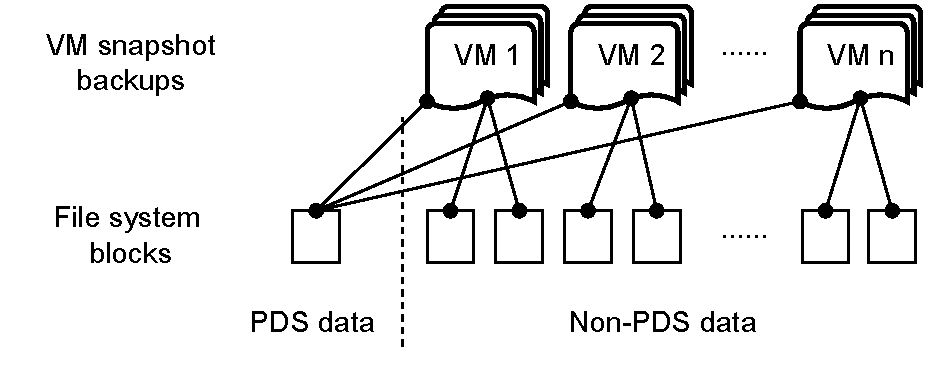
\includegraphics[width=3in]{images/share_vc}
        \label{fig:share_vc}
    }
    \\
    \subfigure[Sharing of file system blocks under VO]
    {
        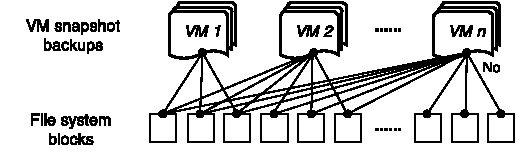
\includegraphics[width=3in]{images/share_vo}
        \label{fig:share_vo}
    }
    \caption{Bipartite association of VMs and file system blocks under (a) VC and (b) VO. }
    \label{fig:share}
\end{figure}

We analyze the impact of replication degree for PDS and non-PDS data items.
The parameters used in our analysis below are defined in Table~\ref{tab:symbol}. 
The replication degree of the backup storage 
is $r$ for regular file system blocks and $r=3$ is a typical setting in distributed
file systems~\cite{googlefs03,hdfs10}.
Since $\sigma$ is small (e.g.  2\% in our experiments),  
the impact of replication on storage increase is very small even 
when choosing  $r_c/r$ ratio as 2 or 3. 


%In the VC approach, a special replication degree $r_c$ is used for PDS data where $r_c>r$. 
%The storage cost for VO with full deduplication is $c_u *r$ and for VC, it is
%$ k*r_c  + (c-E(c-c_u))*r$. Thus The storage cost ratio of $VC$ over $VO$ is 
%\[
%\sigma \frac{r_c}{r} + \frac{c-e(c-c_u)}{c_u}.
%\]
%Since $\sigma$ is small (it is 2\% in our experiments),  
%term $\sigma \frac{r_c}{r}$ is small in the above expression.  
%Thus the impact on storage increase is very small even when we choose a large $r_c/r$ ratio. 
%For example, $r_c/r=2$ or 3. 

Now we  assess  the impact of losing $d$ machines 
to the VC and VO approaches.  
A large $r_c/r$ ratio can have a positive impact on full availability of VM snapshot blocks.
%We use an FSB rather than a deduplication
%data chunk as our unit of failure because the DFS keeps
%file system blocks as its base unit of storage.
To compute the full availability of all snapshots of a VM, we derive
the probability of losing a snapshot FSB of a VM by
estimating the number of file system blocks per VM in each approach.
%As illustrated in Figure~\ref{fig:share},
%we build a bipartite graph representing the association from unique file system blocks
%to their corresponding VMs in each approach. An association edge is  drawn  from an FSB to a VM 
%if this block is used by the VM. 

As illustrated in Figure~\ref{fig:share}, we build a bipartite graph representing the
association from unique file system blocks to their corresponding VMs in the VC
and VO approaches. We use an FSB rather than data chunk as our unit of failure
because the DFS keeps file system blocks as its base unit of storage, and in
the case of 64MB FSBs and 4KB chunks, there are 16K chunks per block. In VC
we assign extra replication to the PDS blocks, while in VO the replication
degree is fixed.

We could consider a third approach (call it VO+), adopting the VO approach, and
then relying on filesystem features to provide extra replication to popular
blocks, without the extra complexity of separating popular and non-popular
data. The problem with this VO+ approach is that without separating the
popular chunks from the less-popular, the popular chunks are dispersed across
all of the filesystem blocks in the storage system. Because the popular blocks
are dispersed, there are very few popular FSBs. The end result is that we
either have to add extra replication on unpopular chunks to ensure the popular
chunks have sufficient replication, or we have to accept a reduced replication
factor on popular chunks. This explains why we must separate the PDS and
non-PDS data in our system to acheive the desired $r_c/r$ ratio (though both
can be stored on the same DFS).

For VC, each VM has an average number $N_1$ of non-PDS FSBs
and  has  an average of  $N_2$ PDS FSBs. 
Each non-PDS FSB is associated with one VM
 and  we denote that PDS FSBs are
shared by an average of $V_c$ VMs. 
%Let $s$ be the average number of chunks per file system block, 
%$V$ be the average number of VMs hosted on each machine. 
Then, 
\[
V pN_1 s  \approx c-E_c(c-c_u) - c_u\sigma\; \mbox{ and } \; 
V pN_2 s  \approx c_u \sigma V_c.
\]

For VO, each VM has an average of $N_o$ FSBs
and let $V_o$ be the average number of VMs shared by each FSB.
\[
V pN_o s  = (c- E_o(c-c_u) ) V_o.
\]

Since each FSB (with default size $64MB$) contains many chunks (on average 4KB),
each FSB contains the hot low-level chunks shared by many VMs, and it also contains
rare chunks which are not shared.  Since $c>> c_u$, from the above equations:
\[
\frac{N_1}{N_o} \approx  \frac{1-E_o}{(1-E_c) V_o}.
\] 
When $E_c$ is close to $E_o$,
%as demonstrated in Section~\ref{sect:evaldedup},
$N_1$ is much smaller than $N_o$. 
%When there is a failure in FSBs with replication degree $r$
%and there is no failure for PDS data with more replicas,   a VM in
%the VC approach has a much lower chance to lose a snapshot than VO. 
%Figure~\ref{fig:fsb-links} shows the average number of VMs sharing each file block from
%our test dataset.
%For VC, we only show
%the sharing degree of  PDS-oriented file blocs  because non-PDS blocks always belong to
%one VM.
%Figure~\ref{fig:fsb-links} shows the average number of VMs sharing each file block from our test data.
Figure~\ref{fig:vm-links} shows the average number of file system blocks for each VM in VC and in VO
and  $N_1$ is indeed  much smaller than $N_o$ in our tested dataset.  
%In fact, $N_1 +N_2 < N_o$. 
%This is likely because the PDS FSBs tightly pack data used by many VMs, 
%which decreases the overall number of FSBs required to backup a VM.
%Note that  if  the backup for multiple VMs were conducted concurrently, there could be many more
%VMs sharing each file block on average in VO. 

%Therefore, even when there is a loss of a PDS block, the VC approach tolerates the fault better.

\comments{
\begin{figure}[htbp]
  \centering
	\begin{tikzpicture}
		\begin{axis}[
                width=\linewidth,
                height=0.6\linewidth,
		%title={VO FSB links},
		xlabel={Number of VMs},
		ylabel={Avg. Num. VMs sharing FSB},
                cycle list name=mline,
                xmin=0,
                ymin=0,
                xmax=106,
		%extra y ticks={4.5,5.5,6.5} %to show extra ticks
		legend pos=north west
		]
                \addplot table[x=VMs,y=FSBLinks] {figures/vo_fsb_links_105.txt};
		\addplot table[x=VMs,y=cdslinks] {figures/cds_links_105.txt};
                \legend{VO, PDS in VC};
		\end{axis}
	\end{tikzpicture}
  \caption{Measured average number of VMs sharing a 64MB FSB in VO and in VC.}
  \label{fig:fsb-links}
\end{figure}

}

\begin{figure}[htbp]
  \centering
	\begin{tikzpicture}
		\begin{axis}[
		%title={VO VM links},
                width=\linewidth,
                height=0.6\linewidth,
		xlabel={Number of VMs},
		ylabel={Avg. Num. FSBs used by VM},
                xmin=0,
                ymin=0,
                xmax=106,
		%extra y ticks={4.5,5.5,6.5} %to show extra ticks
		%legend pos=north east,
                legend style={
                    at={(1,0.825)},
                    anchor=north east
                },
                %legend columns=3
		]
                \addplot[blue,mark=none] table[x=VMs,y=N_O] {figures/vm_links_all.txt};
                %\addplot[red,dotted,mark=none] table[x=VMs,y expr=\thisrow{N_1}+\thisrow{N_2}] {figures/vm_links_all.txt};
                \addplot[red,dashdotted] table[x=VMs,y=N_1] {figures/vm_links_all.txt};
                \addplot[red,densely dashed,mark=none] table[x=VMs,y=N_2] {figures/vm_links_all.txt};
                \legend{$N_o$,
                    %$N_1+N_2$,
                    $N_1$,
                    $N_2$};
		\end{axis}
	\end{tikzpicture}
  \caption{Measured average number of 64MB FSBs used by a single VM. For VC both the number of PDS and Non-PDS FSBs used are shown.}
  \label{fig:vm-links}
\end{figure}

The full snapshot availability of a VM is estimated as follows with parameters $N_1$ and
 $N_2$ for VC and $N_o$ for VO.
Given normal data replication degree $r$, PDS data replication degree $r_c$, 
the availability of a file system block is the probability that  
all of its replicas do not appear in any group of $d$ failed machines among the total of $p$ machines. 
Namely, we define it as
\[
A(r) = 1-\binom{d}{r}/ \binom{p}{r}. 
\]
Then the availability of one VM's snapshot data under VO approach is the probability that
 all its FSBs are unaffected during the system failure:
%\begin{equation}
%\label{eq:VO}
%(1-\frac{ \binom{d}{r}} { \binom{p}{r} })^{N_o}. 
\[
A(r)^{N_o}. 
\]
%\end{equation}

For VC, there are two cases for $d$ failed machines.
\begin{itemize}
\item
When $r \le d<r_c$,  there is no PDS data loss and  
the full snapshot availability of a VM in the VC approach is 
%\begin{equation}
%\label{eq:VC1}
%(1-\frac{\binom{d}{r}} { \binom{p}{r} })^{N_1}.
\[
A(r)^{N_1}.
\]
%\end{equation}
Since $N_1$ is typically much smaller than $N_o$, 
the VC approach has a higher availability of VM snapshots than VO in this case.
%In the evaluation discussed in Section~\ref{sect:evaldedup}, 
%We have considered a worst case scenario where
%every PDS FSB is shared by all VMs in the VC approach, which leads a large $N_2$ value. 
%Even with $N_2$ being much higher than $N_o$ (as discussed below),
%the availability of VC snapshots is much higher than VO.

\item
When $r_c \leq d$, both non-PDS and PDS file system blocks in VC can have a loss.
The full snapshot availability of  a VM in the VC approach is
%\begin{equation}
%\label{eq:VC2}
% (1-\frac{ \binom{d}{r}} { \binom{p}{r} })^{N_1} 
% *
% (1-\frac{ \binom{d}{r_c}} { \binom{p}{r_c} })^{N_2}.
\[
A(r)^{N_1} * A(r_c)^{N_2}.
\]
%\end{equation}
%comparing  Formula~\ref{eq:VO} and~\ref{eq:VC}. 
\end{itemize} 
%In the evaluation discussed in Section~\ref{sect:evaldedup},
We have considered a worst case scenario that
every PDS FSB is shared by all VMs in the VC approach, which leads to a large $N_2$ value. 
Even with that, the availability of VC snapshots is still much higher than VO and  
there are two reasons for this:  1) $N_1$ is much smaller than $N_o$ as discussed previously.
2)  $A(r) < A(r_c)$ because $r < r_c$.  
Table~\ref{tab:fsb-availability} lists the $A(r)$ values with
%that the availability of an individual file system block
different replication degrees, to demonstrate the gap between  $A(r)$ and  $A(r_c)$.

% $1-\frac{ \binom{d}{r}} { \binom{p}{r} } < 1-\frac{ \binom{d}{r_c}} { \binom{p}{r_c} }$

\comments{
\begin{figure}[htbp]
  \centering
    \begin{tikzpicture}
            \begin{axis}[
                width=\linewidth,
                height=0.6\linewidth,
            %title={FSB Availability},
            cycle list name=mline,
            xlabel={Number of Machines Failed},
            ylabel={Availability of Single FSB (\%)},
            %extra y ticks={99.9}, %to add extra ticks
            mark options=solid,
            legend pos=south west,
            %legend columns=2,
            %legend style={
            %    at={(0.5,-0.2)},
            %anchor=north}
            ]
            \addplot table[x=NodesFailed,y=Availability5] {figures/fsb_availability.txt};
            \addplot table[x=NodesFailed,y=Availability4] {figures/fsb_availability.txt};
            \addplot table[x=NodesFailed,y=Availability3] {figures/fsb_availability.txt};
            \legend{$R=5$,$R=4$,$R=3$};
            \end{axis}
    \end{tikzpicture}
    \caption{Availability of a file system block in a 100 machine cluster with different replication 
and failure settings.THIS PLOT WILL BE REPLACED BY TABLE}
  \label{fig:fsb-availability}
\end{figure}
}

\begin{table}
  \centering
    \footnotesize
    \tabcolsep=0.11cm
    \comments{%table data is obsolete, now uses pgfplotstable
        \begin{tabular}{|l|l|l|l|}
        \hline
        \multirow{2}{*}{Failures ($d$)}   & \multicolumn{3}{c|}{$A(r_c)\times 100\%$} \\
                                    %\cline{2-4}
                                    & $r_c=3$ & $r_c=6$ & $r_c=9$ \\
        \hline
        3 & 99.9994 & 100 & 100\\
        5 & 99.9939 & 100 & 100\\
        10 & 99.9258 & 99.9999 & 99.9999 \\
        20 & 99.2950 & 99.9967 & 99.9999 \\
        \hline
    \end{tabular}
    }
    \pgfplotstabletypeset[
        columns={NodesFailed,Availability3,Availability6,Availability9},
        columns/NodesFailed/.style={
            column name={\multirow{2}{*}{Failures ($d$)}}
        },
        columns/Availability3/.style={
            column name={\multicolumn{3}{c|}{$A(r_c) \times 100\%$}\\&$r_c=3$},
            fixed, precision=9
        },
        columns/Availability6/.style={
            column name={$r_c=6$},
            fixed, precision=9},
        columns/Availability9/.style={
            column name={$r_c=9$},
            fixed, precision=9},
        every head row/.style={
            before row={\hline},
            after row={\hline},
        },
        every last row/.style={after row=\hline},
        column type/.add={}{|},
        every first column/.style={column type/.add={|}{}},
    ]{figures/fsb_availability.txt}
    \caption{$A(r_c)$ as storage nodes fail in a 100 node cluster.}
    \label{tab:fsb-availability}
\end{table}


\comments{
\subsection{Impact on Deduplication Efficiency}
Choosing the value $k$ for the most popular chunks affects the deduplication efficiency.
We analyze this impact based on the characteristics  of the VM snapshot traces
studied from  application datasets.
A previous study shows that the popularity of data chunks after local deduplication follows 
a Zipf-like distribution\cite{Breslau1999a} and its
exponent $\alpha$ is ranged between 0.65  and  0.7~\cite{WeiZhangIEEE}. 
Figure~\ref{fig:Datazipf} illustrates the Zipf-like distribution of chunk popularity.
The parameters we will use in our analysis below are defined in
Table~\ref{tab:symbol}. 

%Table~\ref{tab:symbol} defines paramters $c$, $c_u$, $f_i$, and $\delta$ used below.
%let $c$ be the total number of data chunks. 
%$c_u$ be the total number of fingerprints 
%in the global index after complete deduplication, and
%$f_i$ be the frequency for the $i$th most popular fingerprint. 
By Zipf-like distribution, $f_i = {f_1}/{i^\alpha}.$
The total number of chunks in our backup storage which
has local duplicates excluded is $c (1-\delta)$, this can be represented
as the sum of each unique fingerprint times its frequency:
%Since $ \sum_{i=1}^{c_u}f_i = c (1-\delta)$,
\[
f_1 \sum_{i=1}^{c_u}\frac{1}{i^\alpha} = c (1-\delta).
\]
Given $\alpha <1$, $f_1$ can be approximated with integration:
%\begin{equation}
\[
f_1=\frac{c(1-\alpha)(1-\delta)}{c_u^{1-\alpha}}.
\]
%\end{equation}

Thus putting the $k$ most popular fingerprints into PDS index can remove the following number of chunks during global 
deduplication:
\[
f_1 \sum_{i=1}^{k}\frac{1}{i^\alpha} \approx  
f_1 \int_{1}^{k}\frac{1}{x^\alpha} dx  \approx  f_1\frac{  k^{1-\alpha}} {1-\alpha}
=c(1-\delta) \sigma^{1-\alpha}.
\]

Deduplication efficiency of the VC approach using top $k$ popular chunks
is the percentage of duplicates that can be detected:  
\begin{equation}
\label{eq:dedupeff}
%\begin{split}
%e_k &= 
E_c=\frac{ c\delta + c(1-\delta) \sigma^{1-\alpha}}
{c  - c_u }.\\
%\end{split}
\end{equation}

% After the global deduplication, the number of remaining chunks is:
% \[
% c-E(c-c_u)
% \] 

We store the PDS index using a distributed shared memory hash table such as Memcached
and allocate a fixed percentage of memory space per physical machine for top $k$ popular items.
As the number of physical machines ($p$) increases,
the entire cloud cluster can host more VMs; however,  ratio $\sigma$ which is $k/c_u$ remains
a constant because each physical machine on average still hosts a fixed constant number of 
VMs. Then the overall deduplication efficiency of VC defined in Formula~\ref{eq:dedupeff}
remains constant.
Thus the deduplication efficiency is stable  as $p$ increases as long as $\sigma$  is a constant.


\begin{figure}[htbp]
  \centering
    \begin{tikzpicture}
            \begin{axis}[
            %title={PDS Coverage},
            width=\linewidth,
            height=0.6\linewidth,
            cycle multi list={
                mline\nextlist
                [3 of]mmark*\nextlist
            },
            %cycle list name=mcolor,
            xlabel={Total num. chunks stored (in billions)},
            ylabel={PDS Coverage (\%)},
            %extra y ticks={4.5,5.5,6.5} %to add extra ticks
            mark options=solid,
            %legend pos=outer north east,
            legend columns=2,
            legend style={
                at={(0.5,-0.30)},
            anchor=north},
            ]
            \addplot table[x expr=\thisrow{InputChunks}/1000000000,y=A1] {figures/cds_coverage.txt};
            \addplot table[x expr=\thisrow{InputChunks}/1000000000,y=A2] {figures/cds_coverage.txt};
            \addplot table[x expr=\thisrow{InputChunks}/1000000000,y=A4] {figures/cds_coverage.txt};
            \addplot table[x expr=\thisrow{InputChunks}/1000000000,y=T1] {figures/cds_coverage.txt};
            \addplot table[x expr=\thisrow{InputChunks}/1000000000,y=T2] {figures/cds_coverage.txt};
            \addplot table[x expr=\thisrow{InputChunks}/1000000000,y=T4] {figures/cds_coverage.txt};
            \legend{Measured ($\sigma=1\%$),Measured ($\sigma=2\%$),Measured ($\sigma=4\%$),Predicted ($\sigma=1\%$),Predicted ($\sigma=2\%$),Predicted ($\sigma=4\%$)};
            \end{axis}
    \end{tikzpicture}
  \caption{Predicted vs. actual PDS coverage as data size increases.}
  \label{fig:cds-coverage}
\end{figure}
Ratio $\sigma^{1-\alpha}$ represents the percentage of the remaining
chunks detected as duplicates in global deduplication due to PDS.
We call this PDS coverage.
Figure~\ref{fig:cds-coverage} shows predicted PDS coverage using $\sigma^{1-\alpha}$ when $\alpha$ is fixed at
0.65 and measured PDS coverage in our test dataset.
$\sigma=2\%$ represents memory usage of approximately 100MB memory per machine for the PDS.
While the predicted value remains flat, measured PDS coverage increases as more VMs are involved.
This is because the actual $\alpha$ value increases with the data size.
%Then  PDS coverage PDS increases as more VMs are involved.
}

\bibliographystyle{abbrvnat}
\bibliography{library,dedup1}
\end{document}
